\documentclass[british, journal]{IEEEtran}
\usepackage[T1]{fontenc}
\usepackage[latin9]{inputenc}
\usepackage{float}
\usepackage{amsmath}
\usepackage{amssymb}
\usepackage{graphicx}
\usepackage{setspace}
\usepackage{array}
\usepackage{blindtext}

\makeatletter

\newcommand{\noun}[1]{\textsc{#1}}

\@ifundefined{showcaptionsetup}{}{
 \PassOptionsToPackage{caption=false}{subfig}}
\usepackage{subfig}
\makeatother

\usepackage{babel}
\usepackage{algorithmicx}
\usepackage{algpseudocode}
\usepackage{algorithm}

\begin{document}

%\onecolumn
%\section*{Cover letter}
%
%Dear Editors and Reviewers,
%
%\vspace {3mm}
%
%We submit for your review an article entitled "High-level
%asynchronous concepts at the interface between analogue and
%digital worlds", for the Special Issue on Circuit and System
%Design Automation for Internet of Things.
%
%\vspace {3mm}
%
%A previous version of this article was submitted to, and presented
%at the 13th ACM-IEEE International Conference on Formal Methods and
%Models for System Design - MEMOCODE'15 conference. This version is
%available from http://ieeexplore.ieee.org/document/7340478/.
%
%\vspace {3mm}
%
%The additions to the submitted article from the conference paper are
%as follows:
%
%\begin{itemize}
%\item A motivating example, explaining a buck converter controller and
%discussing the existing monolithic design flow used for this.
%
%\item An introduction to interface concepts, a specification for signal
%types composable with all other concepts.
%
%\item A new section discussing interoperability with STG based tools. This
%details an algorithm to translate concepts into STGs, and discusses
%the overall design flow when using concepts.
%
%\item Updated concept specifications for the case study, which are included
%as examples in the concept translation tool, and use the most up to
%date concepts, as described in this article.
%
%\item An updated section on synthesis of a speed-independent controller,
%as part of the case-study. Included is more possible types synthesis,
%the implementation, and their benefits.
%
%\item An expanded section on related work.
%
%\end{itemize}
%
%We thank you in advance for any comments you may give.
%
%\vspace {3mm}
%
%Yours sincerely,
%
%\vspace {3mm}
%
%Jonathan Beaumont, Andrey Mokhov, Danil Sokolov and Alex Yakovlev
%
%\twocolumn

\title{High-level asynchronous concepts at the interface between analogue and 
digital worlds}
\author{Jonathan Beaumont, Andrey Mokhov, Danil Sokolov, Alex Yakovlev\\
\texttt{\{j.r.beaumont, andrey.mokhov, danil.sokolov, alex.yakovlev\}@ncl.ac.uk}\\
\emph{School of Electrical and Electronic Engineering, Newcastle University,
UK}}

\maketitle

\begin{abstract}
Asynchronous circuits are becoming increasingly important in
system design for Internet-of-Things, where they orchestrate
the interface between big synchronous computation components
and the analogue environment, which is inherently asynchronous
and has high uncertainty with respect to power supply,
temperature and long-term ageing effects.
However, wide adoption of asynchronous circuits by industrial users is
hindered by a steep learning curve for asynchronous control models,
such as Signal Transition Graphs, that are developed by the academic
community for specification, verification and synthesis of
asynchronous circuits.

In this article we introduce a novel high-level description language
for asynchronous circuits, which is based on behavioural
\textit{concepts} -- high-level descriptions of asynchronous circuit
requirements, that can be shared, reused and extended by users,
and can be automatically translated to Signal Transition Graphs for
further processing by conventional asynchronous and synchronous EDA tools,
such as \noun{Petrify} and \noun{Mpsat}.
Our aim is to simplify the process of capturing system requirements in the
form of a formal specification, and to promote behavioural concepts as a
means for design reuse. The proposed design flow is fully automated in
open-source toolsuite \noun{Workcraft}, and is applied to the development of
an asynchronous power regulator.
\end{abstract}

\sloppy
\thispagestyle{empty}

\section{Introduction}

Analogue and mixed-signal circuits become more tightly integrated with
digital systems, in particular in mobile and autonomous applications,
such as wearable consumer electronics and self-powered Internet-of-Things
nodes, where it is essential to have intelligent timing control and power
regulation~\cite{7287733}\cite{talbot2016holistic}\cite{6241632}.
An on-chip power management system is an illustrative example: it relies
on analogue circuitry for power regulation and conversion, and its behaviour
is characterised by many operating modes with complex interplay and
high-level decision logic that is digitally controlled.
Asynchronous circuits are event-driven, i.e. they react to changes
in a system at the rate they occur~\cite{sparso2001principles}.
This makes them particularly useful for interacting with analogue world,
where the ability to quickly respond to non-digital input, e.g.
dynamically changing loads across the chip, is essential for reliable
operation and efficiency~\cite{2008_audy_isscc_tutorial}.

Signal Transition Graphs~(STGs)~\cite{Chu_1987_phd}\cite{Rosenblum_1985_tpn}
are commonly used for the specification,
verification and synthesis of asynchronous control circuits as they are
supported by multiple EDA tools, such as \noun{Petrify}~\cite{Cortadella},
\noun{Mpsat}~\cite{khomenko2004detecting}, \noun{Versify}~\cite{i1997formal},
\noun{Workcraft}~\cite{2007_poliakov_workcraft}\cite{Workcraft_website}, and others.
These tools take an STG specification of a complete controller and can
formally verify its correctness, as well as synthesise an asynchronous
circuit implementation that is \emph{speed-independent}, i.e. guaranteed
to work correctly regardless of component delays~\cite{Muller_1959_ts}.
Such a monolithic approach to designing asynchronous circuits has
poor scalability: as the system grows in complexity its monolithic
specification becomes challenging to comprehend and debug. The problem
becomes particularly severe when designing multi-mode systems, such as
power regulators, where capturing all aspects of system behaviour in a
consistent specification is a major design challenge~\cite{2014_sokolov_ftfc}\cite{sokolov2015design}.
The STG models of components and operating modes are difficult to reuse
when designing other specifications, and thus each new design must be built
from the ground up. This further adds to the design time, hence making
asynchronous circuits costly for use in industry.

In this paper we address this issue by proposing a new method for design
of asynchronous circuits based on \emph{behavioural concepts}.
The method splits a specification into several parts corresponding
to operational modes of the circuit (\emph{scenarios}). The features,
constraints and requirements of each scenario (\emph{concepts}),
are described in a formal notation, which we implemented as a domain
specific language embedded in Haskell~\cite{1996_hudak_dsl}. Concepts can
be defined at several levels; specifically, we give examples of signal-,
gate- and protocol-level concepts. It is possible to compose basic concepts
into more complex ones, thus supporting the design reuse at the level of system
specification.
%Commented out as I'm not sure we are actually talking about this in the paper:
%Scenarios of reconfigurable systems~\cite{microadapt}
%can also be parameterised by run-time parameters (e.g., available
%energy budget) or design-time ones (e.g., the number of processing
%cores in a Network-on-Chip network), therefore concepts should also
%support parameterisation.
Concepts can be automatically translated into equivalent STGs and
formally verified using standard tools, e.g. \noun{Workcraft}.
When all scenarios have been translated to STGs and verified, they can be
combined to produce a complete specification, and synthesised into an
asynchronous circuit implementation targeting a chosen technology library.
%Commented out, as this is probably too detailed for the intro.
%This step will also be automated,
%and will offer \emph{templates} for common scenario ordering requirements,
%such as mode switching sequences and start-up scenarios.

Our contributions are as follows:
\begin{itemize}
  \item We introduce asynchronous concepts as a specification
  language in Section~\ref{sec:Concepts} and compare it to STGs in
  Section~\ref{sec:Circuit-specification-with}.
  \item We present an algorithm for translating concepts to STGs
  and integrate it into our open-source software toolsuite \noun{Workcraft},
  Section~\ref{sec:interop-with-stg}.
  \item We demonstrate the proposed design method on a case study of an
  asynchronous power regulator, Section~\ref{sec:case-study}.
\end{itemize}

\noindent
We start with a motivational example in Section~\ref{sec:Motivating Example}, review related work
in Section~\ref{sec:related-work}, and discuss future research in Section~\ref{sec:conclusions}.

%Designing a controller for an analogue circuit using this method can
%be beneficial. Any of the partial knowledge we have about any casual
%relationships between events in the environment can be naturally modelled
%as concepts. When composed with other concepts describing these relationships
%and concepts describing the control which reacts to the environment,
%a model will be produced which shows how the environment and the control
%system interacts.

%The idea is that our approach should reduce the complexity of designing
%asynchronous circuits, so the number of errors should be reduced,
%and easier to find and correct. This will in turn reduce the design
%time, and make asynchronous circuits more desirable for industry, so
%asynchronous circuits can be used in devices more commonly.

%The presented approach is automated as a Haskell tool~\cite{2016_concepts_github}.
%This parses concepts and uses them to produce scenario STGs. We aim to implement
%combination of scenarios in the tool in the future.
%STGs produced, either scenario or full system, are viewed,
%edited, simulated, verified and synthesised using the open-source \noun{Workcraft}
%framework~\cite{2007_poliakov_workcraft}, which features back-end tools \noun{Petrify}
%and \noun{Mpsat} to perform these operations.

%In this paper, we use real life industrial
%example of a buck converter~\cite{2014_sokolov_ftfc} to show our
%design flow, and test this design approach.
%\vspace{-2mm}

\section{Motivating Example: Buck Converter\label{sec:Motivating Example}}

On-chip power management is essential for energy efficiency and reliability of
IoT computation nodes~\cite{7287733}. According to a 2016 report by
Research~\&~Markets, the global power management market will reach \$34.86~billion
by 2022, driven by the increasing demand in various applications, including
traditional IoT sectors such as wearable, automotive, industrial, retail and
building control electronics. Unlike conventional digital components, power
management units need to directly interface with the analogue part of the system
for sensing and controlling it, and can therefore strongly benefit from asynchronous
implementation that allows them to react to changes in the system at the rate
they occur, instead of sampling various analogue parameters by clock, which is
slow and energy-wasteful~\cite{2014_sokolov_ftfc}\cite{sokolov2015design}.
As a compelling example, consider an asynchronous power management controller with
1ns response time to stimuli from the analogue world. To match its performance
with a synchronous equivalent, one would need to clock it at 2-3GHz, as two clock
cycles are required just for a conventional two flip-flop
synchroniser~\cite{2008_kinniment_synchronisation}. Bearing in mind that
power management controllers spend most of their time doing nothing and
waiting for relatively slow changes in the analogue environment, such
a high-speed clock solution would clearly be inadequate.

\begin{figure}[t]
\begin{centering}
\subfloat[\label{fig:buck-schematic}Schematic (digital control in analogue environment).]
{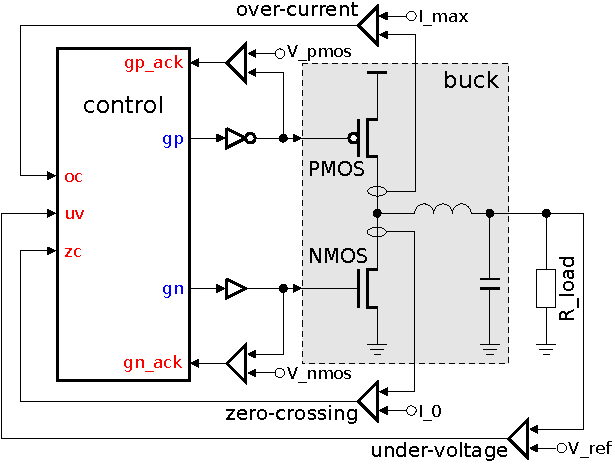
\includegraphics[scale=0.7]{Images/schematic-buck}}
\par
\subfloat[\label{fig:buck-spec}Informal description of three behavioural scenarios.]
{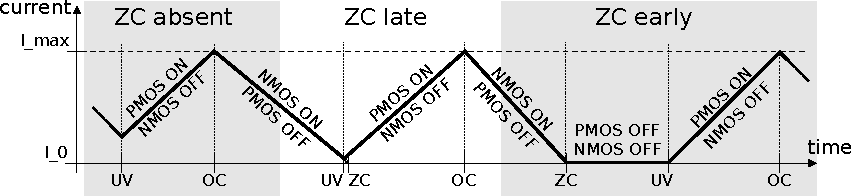
\includegraphics[scale=0.6]{Images/spec-buck}}
\par
\end{centering}
\protect\caption{\label{fig:buck}Buck converter and its informal description.}
\vspace{-3mm}
\end{figure}

In this section we first provide the background on asynchronous buck
converters Section~\ref{sub:buck}, our main motivation example and case study.
Buck converters rely on analogue circuitry for power regulation and
conversion and their behaviour is typically characterised by many operating
modes with complex interplay and high-level decision logic that is digitally
controlled.
We then discuss challenges arising in the design of asynchronous buck converters
with Signal Transition Graphs~(STGs)~\cite{Chu_1987_phd}\cite{Rosenblum_1985_tpn},
a commonly used mathematical model for the specification of asynchronous
circuits Section~\ref{sub:Monolithic}.
Finally, we outline our new design approach Section~\ref{sub:new-way} wherein the
behaviour of an asynchronous buck converter is decomposed into simple
behaviours, that we later refer to as \emph{concepts}. The approach is
described at an intuitive level, and will be formalised in the next
section, Section~\ref{sec:Concepts}.

\subsection{Background on buck converters\label{sub:buck}}

Our motivating example comes from the power management domain, a
\emph{multi-scenario power regulator}~\cite{2014_sokolov_ftfc}.
A basic power regulator comprises an analogue buck and a digital controller,
as shown in Figure~\ref{fig:buck-schematic}. The controller operates
the power regulating PMOS and NMOS transistors of the buck~(using \textsf{$gp$}
and \textsf{$gn$} outputs) as a reaction to \emph{under-voltage}~(UV),
\emph{over-current}~(OC) and \emph{zero-crossing}~(ZC) conditions~(\textsf{$uv$},
\textsf{$oc$}, and \textsf{$zc$} inputs, respectively). These conditions
are detected by a set of sensors that compare the measured current and voltage
with some reference values~(\textsf{V\_ref}, \textsf{I\_max}, \textsf{I\_0}).
Note that in order to avoid a shortcircuit, the PMOS and NMOS transistors of
the buck must never be \noun{On} at the same time. Therefore, the controller
is explicitly notified~(by \textsf{$gp\_ack$} and \textsf{$gn\_ack$})
when the power transistor threshold levels~(\textsf{V\_pmos} and \textsf{V\_nmos})
are crossed.

The operation of a power regulator is usually described in an intuitive,
but rather informal way, e.g. by enumerating the possible sequences
of detected conditions and describing the intended reaction to these
events, as shown in Figure~\ref{fig:buck-spec}. The diagram shows
that UV should be handled by switching the NMOS transistor \noun{Off}
and PMOS transistor \noun{On}, while OC should revert their state~--
PMOS \noun{Off} and NMOS \noun{On}~(\textbf{ZC~absent} scenario). Detection of
the ZC after UV does not change this behaviour~(\textbf{ZC~late} scenario).
However, if ZC is detected before UV then both the PMOS and NMOS transistors
remain \noun{Off} until the UV condition~(\textbf{ZC~early} scenario).

\begin{figure}[t]
\begin{centering}
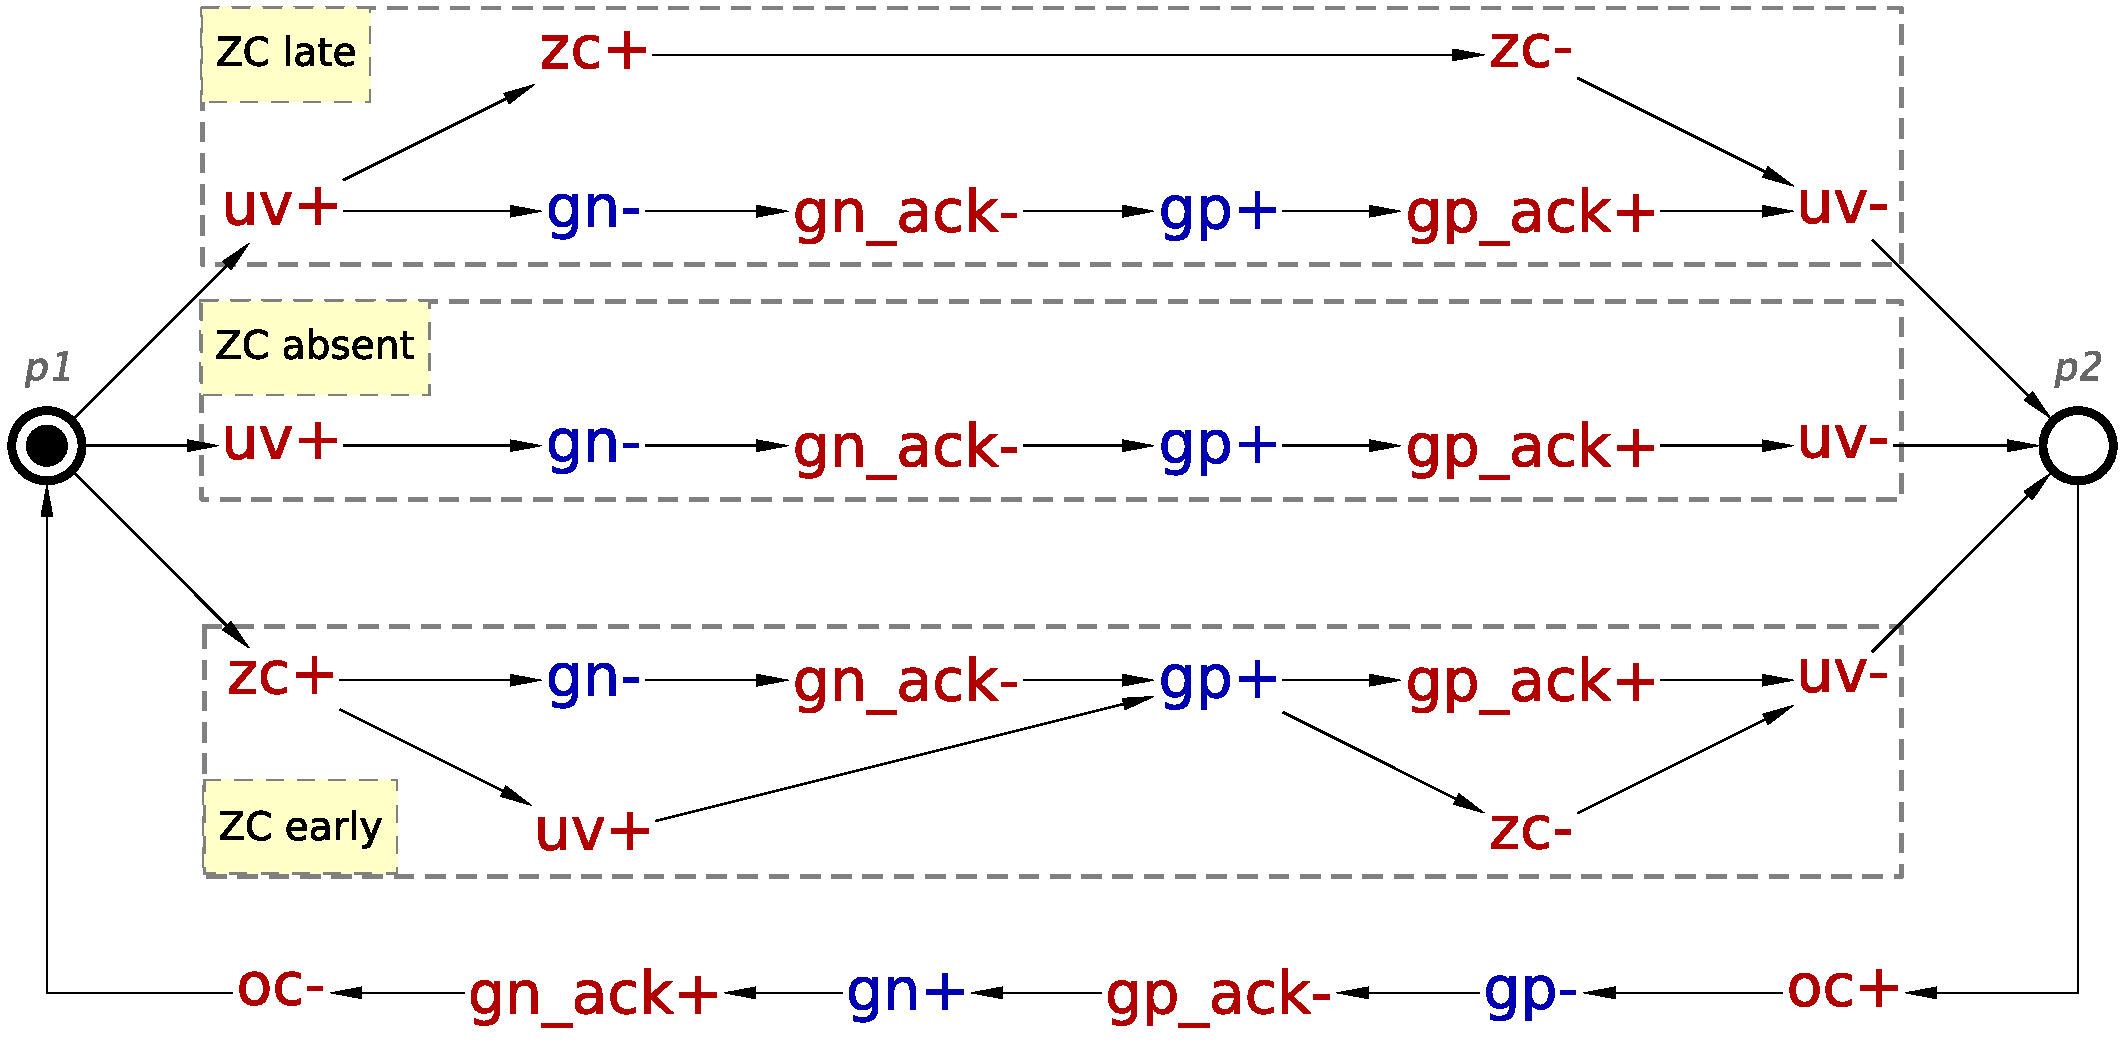
\includegraphics[scale=0.23]{Images/stg-buck}
\par
\protect\caption{\label{fig:Monolithic-buck}STG specification of a simple buck converter.}
\par\end{centering}
\end{figure}

\subsection{Monolithic STG-based design approach\label{sub:Monolithic}}

Using the informal description of three behavioural scenarios, the designer can
produce a formal specification, typically a monolithic STG describing the
complete behaviour of the circuit. Figure~\ref{fig:Monolithic-buck} shows such
a monolithic STG specification for the simple buck controller described above.
Nodes of the STG correspond to signal rising ($+$) and falling ($-$) transitions,
arcs model \emph{causality}, parallel branches correspond to concurrency, and
a circle \emph{place} with a black dot (\emph{token}) represents the choice of
the current scenario. We formally introduce STGs
in Section~\ref{sec:Circuit-specification-with}.

This STG is moderately large and captures all three scenarios by overlaying
their common parts. In the monolithic design approach, the designer starts with
a blank page and manually inserts signal transitions and the connections between
them according to the informal description of the system's operation. With
there being several scenarios, the designer could choose to design each
separately, and then manually compose these taking advantage of the
similarities between the scenarios, as described
in~\cite{2014_sokolov_ftfc}\cite{sokolov2015design}.

In the event that a designer needs to add or remove signals or correct a fault,
editing can become difficult, due to the complexity and size. This can lead to
further faults, and several iterations of design and tests until the new
feature is added and deemed to be working correctly.

A designer may even have to start from a blank page in some cases, unable to
reuse any of the previous design. The larger and more complex an STG is, and
the more signals there are, the more difficult it is to comprehend,
debug and edit. This can slow the design process of a circuit, which is
undesirable in an industry where the time for a device to move from conception
to market is becoming critical, and ever shorter.

\vspace{-2mm}
\subsection{Towards high-level asynchronous concepts\label{sub:new-way}}
In an attempt to streamline the design process, we aimed to find a way to
create STGs which allows editing and reuse at various stages of the design.
This way, if something needs to be corrected, this can be done to a small part,
but we can reuse everything that works correctly. These parts can then be
composed to produce a full STG which contains the corrections, with a minimum
amount of time spent making the corrections.

This led us to take the example of a simple buck converter, and compare what
the STG shows, and what the description of operation of the system, in
particular its signals, is. This allowed us to view interactions between
certain signals which may not be obvious, but without which the STG would not
be a correct representation of the design. For example,
Figure~\ref{fig:stg-breakdown} shows one scenario of the simple buck converter
with some points of interest highlighted.

\begin{figure}[t]
\begin{centering}
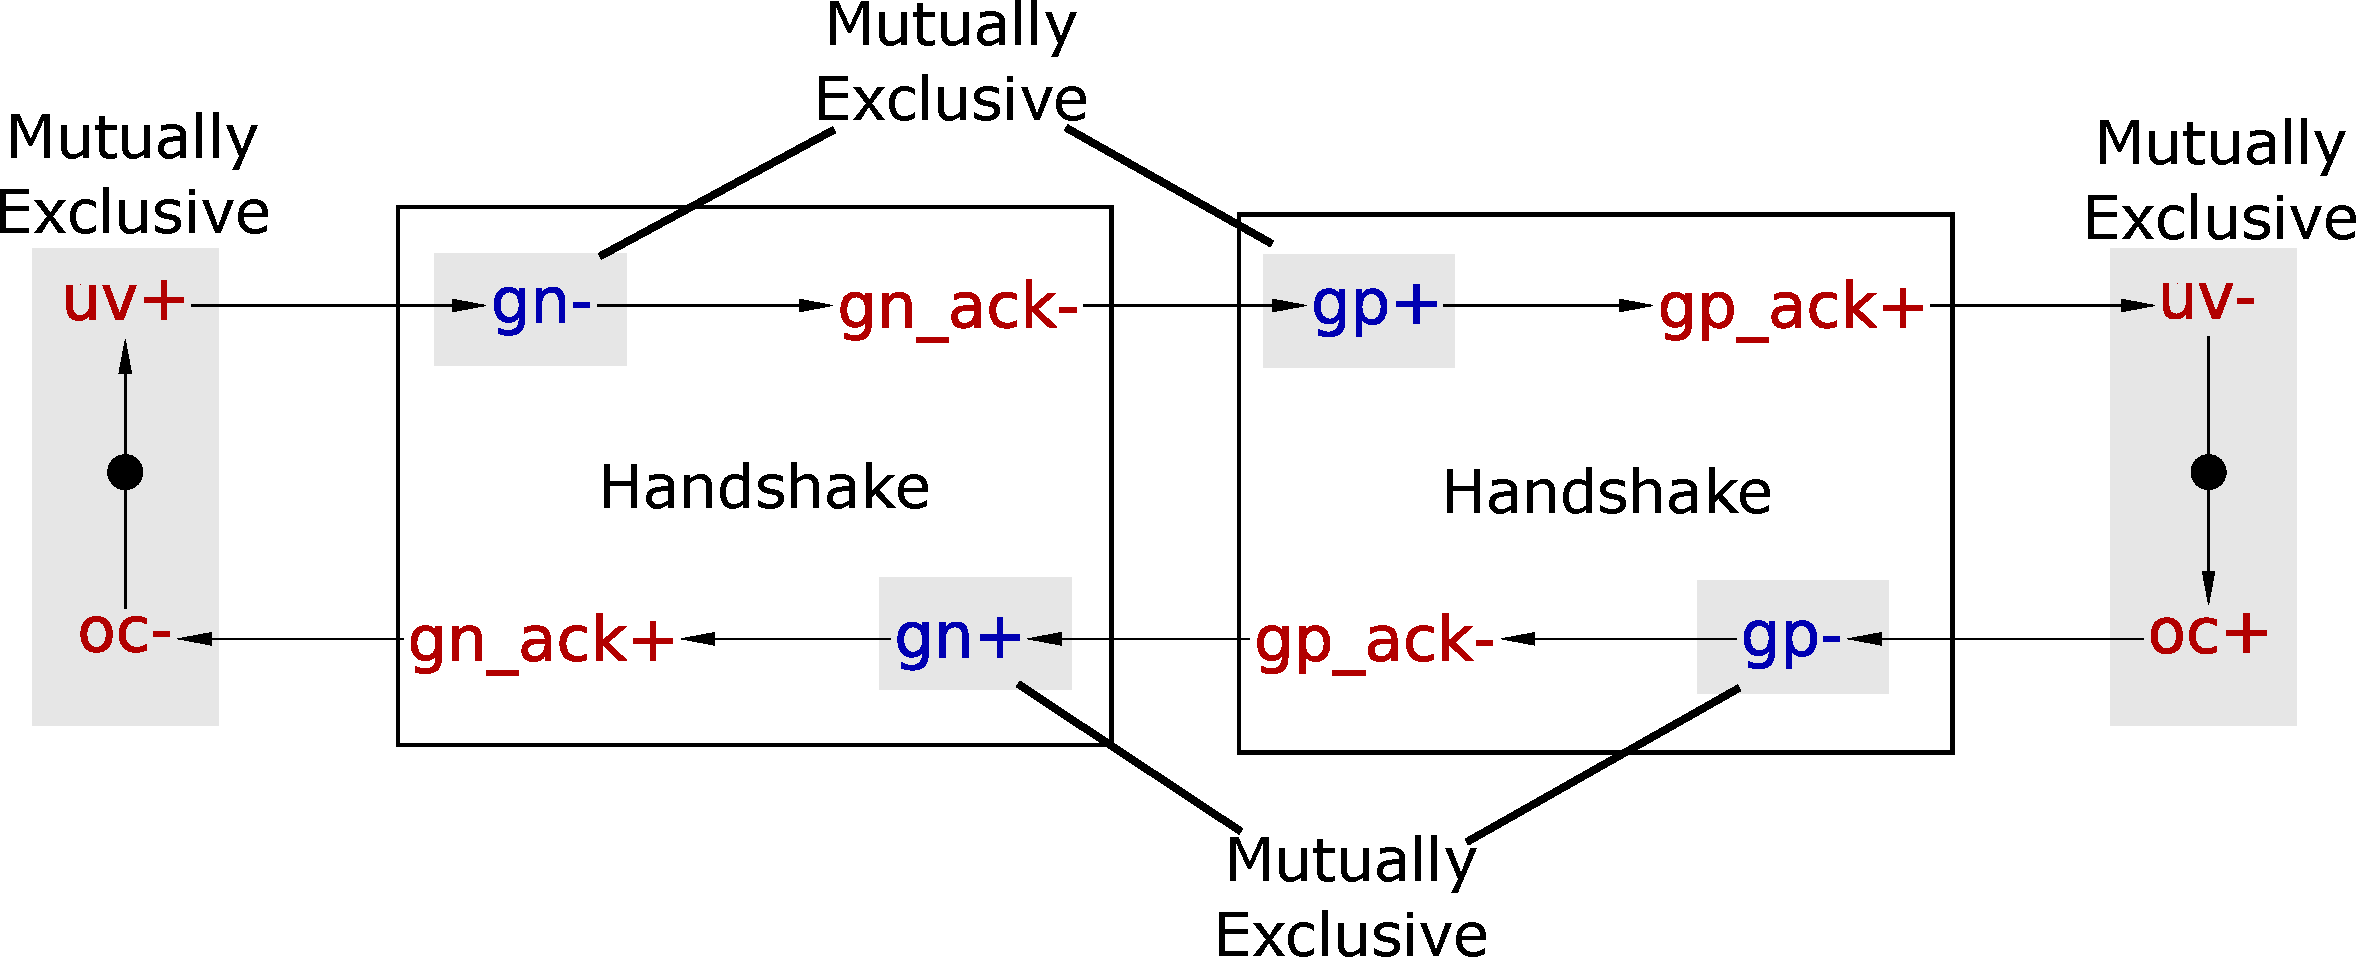
\includegraphics[scale=0.225]{Images/stg-breakdown}
\par
\protect\caption{\label{fig:stg-breakdown}Deconstructing the STG of the ZC absent scenario.}
\par\end{centering}
\vspace{-4mm}
\end{figure}

Studying this STG shows that there are some high-level signal interactions that
we can identify:
\begin{itemize}
\item High levels of $uv$ and $oc$ are mutually exclusive; indeed, $uv$ goes
high (transition $uv^{+}$) only after $oc$ goes low (transition $oc^{-}$), and vice
versa.
\item High levels of $gp$ and $gn$ are also mutually exclusive.
\item Signals $gp$ and $gp\_ack$ form a handshake, i.e. there is a cycle
$gp^{+} \rightarrow gp\_ack^{+} \rightarrow gp^{-} \rightarrow gp\_ack^{-}$ etc.
\item Signals $gn$ and $gn\_ack$ also form a handshake.
\end{itemize}

These interactions can also be identified in the informal buck description:
$uv$ and $oc$ indicate opposite conditions in the circuit and will naturally be
mutually exclusive, while $gp$ and $gn$ are used to switch PMOS and NMOS
transistors respectively, and switching these transistors \noun{On} at the same
time will cause a shortcircuit and is therefore prohibited. Signals $gp\_ack$
and $gn\_ack$ are used to acknowledge the state of these transistors, and thus
always follow $gp$ and $gn$, respectively, forming two separate handshakes.

Knowing this information means that we can describe these protocols once, and
include them in the design of any circuit involving these signals. Any other
interactions between any of these signal will be subject to these protocols,
which will prevent circuit breaking bugs in the testing phase. For example, an
interaction involving $gp$ will ensure that it is never set high at
the same time as $gn$, as otherwise the mutual exclusion will not hold.

If one of these signals is removed, then the protocols that this affects can
be removed, but the unaffected protocols can continue to be used, avoiding a
major re-design which may happen when using the STG-based monolithic approach.

With this idea in mind, we need to find a way to describe these protocols, as
well as other signal interactions, in order to ensure that each different
interaction can be edited without needing to change every single interaction.

%% + Here is the problem we are solving
%%
%%
%%
%%+ STGs are a conventional specification model, STGs tend to get very large and complex for real-life circuits (show simple-buck example STG)
%%
%%
%%
%%+ STGs mix many different concerns in one single graph -- show how one could split the specification into what we call concepts.
%%
\vspace{-2mm}
\section{Concepts \label{sec:Concepts}}

In this section we formally introduce \emph{concepts} that we propose
to employ for the specification of asynchronous circuits. Below we
list (fairly standard) definitions and notational conventions that
are used throughout the paper.

We use $\mathbb{B}$ to denote the set of Boolean values $\{0,1\}$.
Given two Boolean functions $f:X\rightarrow\mathbb{B}$ and $g:X\rightarrow\mathbb{B}$
with the same domain $X$, we lift Boolean operators (disjunction~$\vee$,
conjunction~$\wedge$, implication $\Rightarrow$, etc.) in the usual
manner: $h=f\vee g$ means $h(x)=f(x)\vee g(x)$ for all $x\in X$,
etc. Furthermore,~$\mathbf{0}$ and~$\mathbf{1}$ stand for constant
Boolean functions that discard their input and return $0$
and $1$, respectively.

A \emph{monoid} is a set $M$ and a binary operation $\diamond : M\times M\rightarrow M$
satisfying two axioms:
\begin{itemize}
\item Identity: $e\diamond a=a\diamond e=a$ for any $a\in M$, where $e\in M$
is the \emph{identity element} of the monoid.
\item Associativity: $a\diamond(b\diamond c)=(a\diamond b)\diamond c$ for
all $a,b,c\in M$.
\end{itemize}
Monoid is the simplest mathematical structure that captures the notions
of \emph{emptiness} and \emph{composition}. The concepts introduced
in this section form \emph{commutative monoids}: they have identity
elements corresponding to empty specifications, and can be composed
to build complex concepts from simpler ones. The order of composition
does not matter, i.e., the concepts commute: $a\diamond b=b\diamond a$
for all $a,b\in M$.

\vspace{-1mm}
\subsection{Abstract concepts}

We first describe \emph{abstract concepts} that we use as building
blocks for developing \emph{domain specific concepts}, such as those
related to asynchronous circuits (Section~\ref{sub:Concepts-for-asynchronous}).

Abstract concepts are parameterised by finite sets of \emph{states}
$S$ and \emph{events} $E$. The \emph{initial state concept} captures
all possible (or \emph{permitted}) initial states of the system. In
the most general form it is a function
\[
\mathsf{initial}:S\rightarrow\mathbb{B}
\]
that given a state $s\in S$ returns $1$ if $s$ is an initial state
and $0$ otherwise. In practice this concept is often realised as
a membership test of a set of initial states~$I\subseteq S$, i.e.
$\mathsf{initial}(s)=s\in I$. However, we prefer the functional form
because it is more abstract and permits other, often more efficient
realisations. Note that~$\mathbf{0}$ and~$\mathbf{1}$ have natural
interpretations as initial concepts: they correspond to systems with
no initial states, and systems where any state can be initial, respectively.
Initial state concepts form a commutative monoid with the identity
element~$\mathbf{1}$ and the composition operation~$\wedge$. Intuitively,
if a system comprises two subsystems then its initial state should
satisfy constraints imposed by both subsystems, hence the conjunction
operator.

The \emph{event excitation concept} captures all states wherein a
given event can occur (or is \emph{excited}). In the most general
form it is a function
\[
\mathsf{excited}:E\times S\rightarrow\mathbb{B}
\]
that given an event $e\in E$ and a state $s\in S$ checks whether
$e$ is excited in $s$. In practice this concept is often realised
using \emph{interpreted graph models} such as Finite State Machines
and Petri Nets~\cite{Cortadella}, STGs, Conditional Partial Order
Graphs~\cite{CPOG1}, and others. A partial application of the excitation
function is often useful: $\mathsf{excited}(e)$ captures all states where
event $e$ is excited; for example, if $\mathsf{excited}(e)=\mathbf{0}$ then
$e$ is never excited or \emph{dead}. Event excitation concepts also
form a commutative monoid with~$e=\mathbf{1}$ and~$\diamond=\wedge$.
This definition corresponds to the \emph{parallel composition} operation,
a standard notion for many behavioural models~\cite{PCOMP}.

Some states may be impossible or undesirable during the normal system
operation. To express this we use the \emph{invariant concept}, which
captures all \emph{correct} or \emph{permitted} states of the system.
A typical use case for invariant concepts is to specify assertions
or assumptions about the system state space, that may by verified
via model checking and/or used for optimising the implementation.
In the most general form an invariant concept is a function
\[
\mathsf{invariant}:S\rightarrow\mathbb{B}
\]
that given a state $s\in S$ returns $1$ if $s$ is permitted by
the invariant and $0$ otherwise. Note that if for some state $s$
the initial concept $\mathsf{initial}(s)$ holds but the invariant
$\mathsf{invariant}(s)$ does not hold, then the specification is
\emph{contradictory} and cannot be satisfied by any implementation.
We therefore usually assume that $\mathsf{initial}(s)\Rightarrow\mathsf{invariant}(s)$
holds for all $s\in S$. Similarly, invariant concepts form a commutative
monoid with~$e=\mathbf{1}$ and~$\diamond=\wedge$. Intuitively,
if a system comprises two subsystems then its states should be permitted
in both of the subsystems.

One can derive other useful concepts from the three concepts described
above, for instance,
\[
\mathsf{silent}(e,s)=\overline{\mathsf{excited}(e,s)}
\]
captures all states $s\in S$ when a given event $e\in E$ cannot
occur. Furthermore, one can define other useful concepts that cannot
be derived from the above, e.g., the \emph{execution concept} capturing
the effects that different events have on the system state. Due to
space limitations we only consider the three concepts defined above
and their derivatives.

All the above concepts are monoids, hence their combinations are
trivially monoids too. It is convenient to consider triples
of concepts $(\mathsf{initial},\mathsf{excited},\mathsf{invariant})$
with $(\mathbf{1},\mathbf{1},\mathbf{1})$ representing the \emph{empty
specification}, and composition
$(\mathsf{initial}_{1},\mathsf{excited}_{1},\mathsf{invariant}_{1})\diamond(\mathsf{initial}_{2},\mathsf{excited}_{2},\mathsf{invariant}_{2})$
defined as
$(\mathsf{initial}_{1}\diamond\mathsf{initial}_{2},\mathsf{excited}_{1}\diamond\mathsf{excited}_{2},\mathsf{invariant}_{1}\diamond\mathsf{invariant}_{2})$.
Note that composition of two non-contradictory specifications is
always non-contradictory, that is if both $\mathsf{initial}_{1}(s)\Rightarrow\mathsf{invariant}_{1}(s)$
and $\mathsf{initial}_{2}(s)\Rightarrow\mathsf{invariant}_{2}(s)$
hold for all states $s\in S$, then $\mathsf{initial}_{1}(s)\diamond\mathsf{initial}_{2}(s)\Rightarrow\mathsf{invariant}_{1}(s)\diamond\mathsf{invariant}_{2}(s)$
holds too.

%\vspace{-3mm}



\subsection{Concepts for asynchronous circuits\label{sub:Concepts-for-asynchronous}}

%\vspace{-2mm}


We now introduce concepts which are specific for the domain of asynchronous
circuits and express them using the abstract concepts defined above.

\textbf{\label{signal-level}Signal-level concepts:} States and events of an asynchronous
circuit are parameterised by a set of signals $A$. A state
$s\in S$ is an assignment of Boolean values to signals, i.e. a function
$s:A\rightarrow\mathbb{B}$, while an event $e\in E$ is a \emph{signal
transition}, i.e. a pair $e:A\times\mathbb{B}$ comprising a signal
$a\in A$ and the value of the signal \emph{after} the transition
occurs. We call transitions $(a,0)$ and $(a,1)$ \emph{falling} and
\emph{rising}, respectively, and denote them by $a^{-}$ and $a^{+}$
for brevity.

The following two predicates are very useful for constructing concepts:
\[
\begin{array}{ccc}
\mathsf{before} & \!\!\!\!:\!\!\!\!\! & E\times S\rightarrow\mathbb{B}\\
\mathsf{after} & \!\!\!\!:\!\!\!\!\! & E\times S\rightarrow\mathbb{B}
\end{array}
\]
A state $s\in S$ is said to be \emph{before} a transition $(a,b)\in E$
if $s(a)\neq b$, i.e. in state $s$ signal $a$ has a value which
is different from the resulting value of the transition. Similarly,
$s$ is \emph{after} $(a,b)$ if $s(a)=b$ (the transition has already
occurred).

We are now ready to define an excitation concept called \emph{consistency}~\cite{Cortadella}:
\[
\mathsf{consistency}=\mathsf{before}
\]
This concept captures the requirement that in a consistent asynchronous
circuit a signal transition can only be excited in states that are
before it.

Another key concept in asynchronous circuits is \emph{causality}:
we say that a transition $\mathit{effect}\in E$ causally depends
on transition $\mathit{cause}\in E$, denoted as
\[
\mathsf{causality}(\mathit{cause},\mathit{effect}):E\times E\rightarrow\mathbb{B}
\]
 if $\mathit{effect}$ can occur only in states that are after $\mathit{cause}$.
This is an excitation concept, which can be expressed as follows:
\[
\mathsf{causality}(\mathit{cause},\mathit{effect})(e)\!=\!\begin{cases}
\mathbf{1} & \mathit{if}\, e\neq\mathit{effect}\\
\mathsf{after}(cause) & \mathit{otherwise}
\end{cases}
\]
In words, we do not add any constraints to events $e\in E$ that are
distinct from $\mathit{effect}$, but $\mathit{effect}$ is constrained
to occur only after $\mathit{cause}$. Note that function $\mathsf{after}$
is used in the partially applied form. We will use a short-hand notation
\[
\mathit{cause}\rightsquigarrow\mathit{effect}
\]
for the causality concept for convenience.
% TODO: Maybe bring back later.
% While this concept is called \emph{causality}, this doesn't necessarily imply timings, such as any $\mathit{cause}$ transition immediately forcing the
% $\mathit{effect}$ transition it applies to. Causality can be used in order to list all possible $\mathit{cause}$ transitions which need to occur in order
% for an $\mathit{effect}$ transition.
One can compose two causality concepts using the monoid composition.
\[
a\rightsquigarrow c\ \diamond\ b\rightsquigarrow c
\]
corresponds to so-called AND-causality: event $c$ can only occur
after both $a$ and $b$ have occurred. Specifying OR-causality is
slightly more tricky:
\[
\mathsf{orCausality}(a,b,c)(e)=\begin{cases}
\mathbf{1} & \mathit{if}\, c\neq\mathit{e}\\
\mathsf{after}(a)\vee\mathsf{after}(b) & \mathit{otherwise}
\end{cases}
\]
Event $c$ is thus excited after at least one cause has occurred.

\textbf{Gate-level concepts:} Using the causality concept we can express
the behaviour of gates in asynchronous circuits. For example, a \emph{buffer}
is a gate with one input signal $a\in A$ and one output signal $b\in A$,
whose output transitions causally depend on the input ones:
\[
\mathsf{buffer}(a, b)=a^{+}\rightsquigarrow b^{+}\ \diamond\ a^{-}\rightsquigarrow b^{-}
\]

An \emph{inverter} has a similar conceptual specification, but the
output transition is inverted:
\[
\mathsf{inverter}(a, b)=a^{+}\rightsquigarrow b^{-}\ \diamond\ a^{-}\rightsquigarrow b^{+}
\]
% TODO: Maybe bring this back.
% An \emph{SR-Latch} has two input signals, $s$ and $r$ each of which cause differing transitions with the output, $q$:
% \[
% \mathsf{SRLatch}\,s \,r \,q=s^{+}\!\rightsquigarrow\! q^{+}\ \diamond\ r^{+}\!\rightsquigarrow\! q^{-}\ \diamond\ s^{-}\!\rightsquigarrow\! q^{-}\ \diamond\ r^{-}\!\rightsquigarrow\! q^{+}
% \]
% This can be described as, the\emph{set} signal, $s$ when active, or high, will cause the gate to latch a high state, outputting this with signal $q$ being high. Conversely, the \emph{reset} signal, $r$, when active, or high, will cause the gate to latch a low state, and the output $q$ will be low in this case.
% Another way of specifying this gate using concepts is to use the buffer and inverter concepts defined above, as the signals $s$ and $q$ have an interaction the same as a buffer, and signals $r$ and $q$ interaction is the same as an inverter.
% \[
% \mathsf{SRLatch}\,s \,r \,q=\mathsf{buffer}\,s \,q \ \diamond\ \mathsf{inverter}\,r \,q
% \]

An \emph{AND gate} has two inputs $a$ and $b$ and one output~$c$, which
synchronises rising transitions via AND-causality and falling transitions
via OR-causality:
\[
\mathsf{and}(a, b, c)=a^{+}\!\rightsquigarrow\!c^{+} \diamond\ b^{+}\!\rightsquigarrow\! c^{+} \diamond\ \mathsf{orCausality}(a^{-},b^{-},c^{-})
\]

A \emph{C-element} is a gate with two inputs $a$ and $b$ and one
output~$c$, which synchronises both rising and falling input transitions
via AND-causality (see an example in Section~\ref{sub:Comp-of-concepts}):
\[
\mathsf{cElement}(a, b, c)=a^{+}\!\rightsquigarrow\! c^{+}\ \diamond\ b^{+}\!\rightsquigarrow\! c^{+}\ \diamond\ a^{-}\!\rightsquigarrow\! c^{-}\ \diamond\ b^{-}\!\rightsquigarrow\! c^{-}
\]
% In words, the rising output transition $c^{+}$ causally depends on
% both $a^{+}$ and $b^{+}$, and the falling output transition $c^{-}$
% causally depends on both $a^{-}$ and $b^{-}$.
An alternative way to express the same concept is to reuse the buffer concept:
\[
\mathsf{cElement}(a, b, c)=\mathsf{buffer}(a, c) \diamond \mathsf{buffer}(b, c)
\]
Indeed, a C-element combines the constraints imposed on the output
transitions by two `virtual' buffers.

Behaviour of other gates can be similarly defined using concepts,
see our open-source implementation~\cite{2016_concepts_github}.

\textbf{Protocol-level concepts:} In addition to gate-level concepts
described above it is often important to specify \emph{protocols}
of interaction between multiple gates, components or signals, as
discussed in the motivating example Section~\ref{sub:new-way}.

Here we demonstrate how one can use concepts to specify asynchronous handshakes
and mutual exclusion mechanisms.

Given two signals $a$ and $b$, a \emph{handshake} between them is
the following composition of causality concepts:
\[
\mathsf{handshake}(a, b)=a^{+}\!\rightsquigarrow\! b^{+}\ \diamond\ b^{+}\!\rightsquigarrow\! a^{-}\ \diamond\ a^{-}\!\rightsquigarrow\! b^{-}\ \diamond\ b^{-}\ \rightsquigarrow\! a^{+}
\]
Intuitively, we have a two-way asynchronous communication channel,
where one party sends transitions $a^{+}$ and $a^{-}$ and the other
party responds by corresponding $b^{+}$ and $b^{-}$ transitions.
One can notice that the four causality concepts match those found
in the buffer and inverter concepts, which leads to an alternative
way to express a handshake between~$a$ and~$b$:
\[
\mathsf{handshake}(a, b)=\mathsf{buffer}(a, b) \diamond\mathsf{inverter}(b, a)
\]
Indeed, this conceptual understanding of a handshake as being composed
from a buffer and an inverter is often used by circuit designers as
a convenient way of reasoning.

In order to specify the initial state of a handshake between signals~$a$
and~$b$, we use the $\mathsf{initialise}$ concept:
\[
\mathsf{initialise}(\mathit{signal},\mathit{value})=\mathsf{after}(signal, value)
\]

\noindent For example, $\mathsf{initialise}(a, 0)$ sets the state of the signal
$a$ to $0$. We can compose an initial state concept with the handshake concept
into a combined $\mathsf{handshake00}(a, b)$ concept as
\[
\mathsf{handshake}(a, b) \diamond \mathsf{initialise}(a, 0) \diamond \mathsf{initialise}(b, 0)
\]
The resulting concept corresponds to a handshake between signals~$a$
and~$b$ that are both initially $0$.

The last important concept that requires an introduction is \emph{mutual
exclusion} between two signals~$a$ and~$b$:
\[
\mathsf{me}(a, b) = a^{-}\rightsquigarrow b^{+}\ \diamond\ b^{-}\rightsquigarrow a^{+}\diamond\overline{\mathsf{after}\,a^{+} \, \wedge\mathsf{after}\,b^{+}\, }
\]
The concept comprises two parts: i) in terms of causality, we say
that rising transitions $a^{+}$ and $b^{+}$ can only occur after
the opposite falling ones, ii) the initial states when $a=b=1$ are
forbidden. Taken together these parts guarantee that $a$ and
$b$ are never set to $1$ at the same time, i.e. they are mutually
exclusive. We also add $\overline{\mathsf{after}\, a^{+} \, \wedge\mathsf{after}\ b^{+}\,}$
to the invariant.

We can now specify a \emph{mutual exclusion element}~\cite{2008_kinniment_synchronisation}
that receives asynchronous requests $r_{1}$ and $r_{2}$ to a shared
resource and grants access to it by corresponding mutually exclusive
signals $g_{1}$ and $g_{2}$:

\vspace{-3mm}
{\small
\[
\mathsf{meElement}(r_{1}, r_{2}, g_{1}, g_{2})\!=\!\mathsf{buffer}(r_{1}, g_{1}) \diamond \mathsf{buffer}(r_{2}, g_{2}) \diamond \mathsf{me}(g_{1}, g_{2})
\]}
\vspace{-3mm}

\textbf{Interface concepts:} To specify the type of a signal (\emph{input},
\emph{output} or \emph{internal}) we introduce the \textsf{interface} concept:
\[
\mathsf{interface} : A \rightarrow \{\mathsf{Input}, \mathsf{Output}, \mathsf{Internal}\}
\]
Signal types are composed according to the following rules:
\[
\begin{array}{|l||l|l|l|}
\hline
\multicolumn{1}{|c||}{\diamond} & \mathsf{Input}    & \mathsf{Output}   & \mathsf{Internal} \\ \hline \hline
\mathsf{Input}   & \mathsf{Input}    & \mathsf{Output}   & \mathsf{Internal} \\ \hline
\mathsf{Output}  & \mathsf{Output}   & \mathsf{Output}   & \mathsf{Internal} \\ \hline
\mathsf{Internal}& \mathsf{Internal} & \mathsf{Internal} & \mathsf{Internal} \\ \hline
\end{array}
\]
The intuition is as follows:
\begin{itemize}
    \item If a signal is an input in one component of the system, but is an
    output in another components, then in the composition it will be an output.
    \item An internal signal is similar to an output signal in the sense
    that it is driven by the circuit (not the environment), but it is hidden, i.e.
    not accessible via the circuit interface. Once a signal is hidden and declared
    internal it cannot be revealed.
\end{itemize}

\noindent Specifying signal types is important when designing asynchronous
circuits, as it helps to quickly identify errors (e.g. an input transition is
caused by a hidden internal transition), and reuse existing tools for circuit
simulation, verification and synthesis. Signal type information is also used
in the algorithm for automated translation of concepts to
STGs (Section~\ref{sec:interop-with-stg}).

Concepts \textsf{inputs}, \textsf{outputs}, \textsf{internals} are defined for
specifying types of sets of signals for convenience. For example, to specify
that signals $a$ and $b$ are inputs, $c$ is an output, and $t$ is internal, it
is possible to write:
\[
\mathsf{inputs}(\{a, b\}) \diamond \mathsf{outputs}(\{c\}) \diamond \mathsf{internals}(\{t\}).
\]

\section{Circuit specification with concepts \label{sec:Circuit-specification-with}}

%\vspace{-2mm}

Here we present a method for deriving a circuit specification
from a set of concepts that describe its different aspects. We focus
on specification of \emph{speed-independent}~(SI) circuits, which
is an important class of asynchronous circuits~\cite{Muller_1959_ts}
that work correctly regardless of the gate delays, while the wires
are assumed to have negligible delays. Alternatively, one can regard
wire forks as isochronic and add wire delays to the corresponding
gate delays~(\emph{Quasi-Delay Insensitive}~(QDI) circuit class~\cite{Martin_1986_dc}).
A convenient formalism for specification of SI circuits is
STGs~\cite{Chu_1987_phd}\cite{Rosenblum_1985_tpn},
which is a special kind of Petri nets~\cite{Petri_1962_phd} whose
transitions are associated with signal events.

\vspace{-1mm}
\subsection{Petri nets and STGs}

Formally, a Petri net is defined as a tuple~$PN=\left\langle P,\, T,\, F,\, M_{0}\right\rangle $
comprising finite disjoint sets of \emph{places~}$P$ and \emph{transitions~}$T$,
\emph{arcs} denoting the flow relation~$F\subseteq\left(P\times T\right)\cup\left(T\times P\right)$
and \emph{initial~marking~}$M_{0}$. There is an arc between~$x\in P\cup T$
and~$y\in P\cup T$ iff $\left(x,y\right)\in F$. The \emph{preset}
of a node $x\in P\cup T$ is defined as $\bullet x=\left\{ y\mid\left(y,x\right)\in F\right\} $,
and the \emph{postset} as $x\bullet=\left\{ y\mid\left(x,y\right)\in F\right\} $.
The dynamic behaviour of a Petri net is defined as a \emph{token~game},
changing marking according to the enabling and firing rules. A \emph{marking}
is a mapping~$M:\, P\rightarrow\mathbb{N}$ denoting the number of
\emph{tokens} in each place~($\mathbb{N}=\left\{ 0,1\right\} $ for
\emph{1-safe} Petri nets). A transition $t$ is \emph{enabled} iff
$\forall p,p\in\bullet t\Rightarrow M(p)>0$. The evolution of a Petri
net is possible by \emph{firing} the enabled transitions. \emph{Firing}
of a transition~$t$ results in a new marking $M'$ such that
\[
\forall p~M'(p)=\left\{ \begin{array}{ll}
M(p)-1 & \textit{if}\, p\in\bullet t\setminus t\bullet,\\
M(p)+1 & \textit{if}\, p\in t\bullet\setminus\bullet t,\\
M(p)\,\,\,\,\, & \textit{otherwise}.
\end{array}\right.
\]

An STG is a 1-safe Petri net whose transitions are labelled by signal
events, i.e. $STG=\left\langle P,\, T,\, F,\, M_{0},\,\lambda,\, Z,\, v_{0}\right\rangle $,
where $\lambda$ is a \emph{labelling~function}, $Z$ is a set of
\emph{signals} and $v_{0}\in\left\{ 0,\,1\right\} ^{\left|Z\right|}$
is a \emph{vector~of}~\emph{initial~signal~values}. The labelling
function $\lambda:T\rightarrow Z^{\pm}$ maps transitions into \emph{signal~events}
$Z^{\pm}=Z\times\left\{+,-\right\}$. The signal events labelled $z^{+}$
and $z^{-}$ denote the transitions of signals $z\in Z$ from 0~to~1~(rising
edge), or from 1~to~0~(falling edge), respectively. The labelling
function does not have to be 1-to-1, i.e. transitions with the same
label may occur several times in the net. To distinguish transitions
with the same label and refer to them from the text an index $i\in\mathbb{N}$
is attached to their labels as follows: $\lambda\left(t\right)/i$,
where $i$ differs for different transitions with the same label.
STGs inherit the operational semantics of their underlying PNs, including
the notions of transition enabling and firing.

Graphically, the places are represented as circles, transitions as
text labels, arcs are shown by arrows, and tokens are depicted by dots.
For simplicity, the places with one incoming
and one outgoing arc are often hidden, allowing arcs~(with implicit
places) between transitions.

\begin{figure}[t]
\begin{centering}
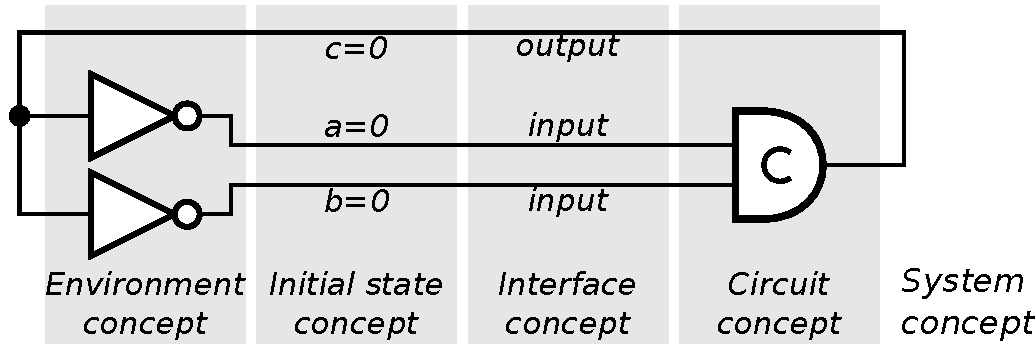
\includegraphics[scale=0.51]{Images/C-element-with-environment}
\par\end{centering}
\vspace{-1mm}
\protect\caption{\label{fig:cElement-concepts}Example system specified using concepts.}
\vspace{-5mm}
\end{figure}

\vspace{-1mm}
\subsection{Composition of concepts\label{sub:Comp-of-concepts}}

A single concept can be used to describe an initial state, invariant
states, a single event or a combination of these, yet describing some
protocols using this method can become long winded, as these can involve
multiple events. We make use of the monoid composition of concepts
to describe complex systems incrementally. Importantly we can mix
several levels of system description and refer to signal, gate and
protocol level concepts in one specification, depending on which level
is more convenient in a particular situation.

Consider an example of a C-element, which has signals $a$ and $b$ as inputs,
and signal $c$ is the output. The output of this C-element is connected to
each of the inputs via an inverter. This is a simple example of a complete
system, of a C-element with an environment, see Figure~\ref{fig:cElement-concepts}.
The example can be described by the following script:

\vspace{-3mm}
\[
\begin{array}{lcl}
\mathsf{circuit}(a,b,c)&\hspace{-2mm}=&\hspace{-2mm}\mathsf{interface}~\diamond~\mathsf{outputRise}~\diamond~\mathsf{inputFall}\\
~&\hspace{-2mm}\diamond&\hspace{-2mm}\mathsf{outputFall}~\diamond~\mathsf{inputRise}~\diamond~\mathsf{initialState}\\
\mathsf{where}&~&\\
\,\,\,\,\,\,\mathsf{interface}&\hspace{-2mm}=&\hspace{-2mm}\mathsf{inputs}(\{a,b\})\diamond\mathsf{outputs}(\{c\})\\
\,\,\,\,\,\,\mathsf{outputRise}&\hspace{-2mm}=&\hspace{-2mm}\,a^{+}\rightsquigarrow c^{+}\,\diamond\, b^{+}\rightsquigarrow c^{+}\\
\,\,\,\,\,\,\mathsf{inputFall}&\hspace{-2mm}=&\hspace{-2mm}c ^ {+} \rightsquigarrow a^{-} \diamond\, c ^ {+} \rightsquigarrow b^{-}\\
\,\,\,\,\,\,\mathsf{outputFall}&\hspace{-2mm}=&\hspace{-2mm}a^{-} \rightsquigarrow c^{-} \,\diamond\, b^{-} \rightsquigarrow c^{-}\\
\,\,\,\,\,\,\mathsf{inputRise}&\hspace{-2mm}=&\hspace{-2mm}c^{-} \rightsquigarrow a^{+} \,\diamond\, c^{-} \rightsquigarrow b^{+}\\
\,\,\,\,\,\,\mathsf{initialState}&\hspace{-2mm}=&\hspace{-2mm}\mathsf{initialise}(a,0) \diamond \mathsf{initialise}(b,0) \\
&~&\hspace{-4.3mm}\diamond \, \mathsf{initialise}(c,0)\\
\end{array}
\]

The first concepts in this list is the \textsf{circuit} concept, defined as a
composition of the following five listed after the \textsf{where} keyword.
They describe certain aspects of the system: the first four are named
according to what they represent, for example, \textsf{outputRise} describes
the events which cause the output to rise, and the final concept defines
the initial states.

%The sixth concept composes all of the first
%5 concepts, and can be translated to the STG shown in Figure~\ref{fig:cElement STG composition}.
%The first four are named according to what they represent, for example,
%\textsf{\textit{\emph{outputRise}}}\textit{ }describes the events
%which cause the output to rise\textit{.} The fifth concept is the
%initial state concept. This is necessary for the algorithm to produce
%a scenario STG, as the STG produced will not be usable without knowing
%the states the signals will be in when the scenario is entered. The
%algorithm takes this concept and works out where tokens need to be
%placed in the STG produced.

Note: For better readability the format of concept scripts used in the article
differs from the actual syntax used in our current implementation, which is
embedded in Haskell programming language~\cite{1996_hudak_dsl} and therefore
relies on the standard Haskell syntax. The basis of the format used here is the
same, but there are some minor differences. An up-to-date description of the
actual syntax supported by the developed tool can be found in the
manual~\cite{2016_concepts_github}.

%Note: The code demonstrated in this example is the format required to work with the tool.
%For the purpose of clarity, in this document we will be changing some of the syntax when defining concepts.
%We will omit the module declaration, and imports, as well as
%the declaration of types for \emph{circuit}, as these are required, and as such will be included in all concepts.
%\emph{rise} and \emph{fall} are used in the code to represent a high and low transition respectively.
%We replace \emph{rise} with '+' and \emph{fall} with '-'. Finally, the diamond composition operator in code is both a '<' and '>' as
%a diamond character is not a standard keyboard character. In this article, we will use $\diamond$ to denote composition.
%All examples in this article are available in the
%format used by the tool from it's GitHub repository~\cite{2016_concepts_github}.

This set of concepts is only one way of describing this C-element
and the environment. Another way could be to use gate-level concepts
and describe the environment explicitly. In this case the environment
allows the inputs to transition in the opposite direction to the output
$c$, as two inverters would. We can then compose this with the C-element
and the same \textsf{interface} and \textsf{initialState} concepts as follows:

\vspace{-3mm}
\[
\begin{array}{lcl}
\mathsf{circuit}(a,b,c)&\hspace{-2mm}=&\hspace{-2mm}\mathsf{interface}~\diamond~\mathsf{cElement}(a,b,c)\\
~&\hspace{-2mm}\diamond&\hspace{-2mm}\mathsf{environment}\diamond\mathsf{initialState}\\
\mathsf{where}&~&~\\
\,\,\,\,\,\,\mathsf{environment}&\hspace{-2mm}=&\hspace{-2mm}\mathsf{inverter}(c,a)~\diamond~\mathsf{inverter}(c,b)
\end{array}
\]

\noindent This specification is equivalent to the previous one; indeed one can
prove this by rearranging the primitive concepts using the commutativity
and associativity of the underlying commutative monoid. Consequently,
this specification will be translated to the same STG shown in
Figure~\ref{fig:cElement STG composition}.

\begin{figure}[h]
\begin{centering}
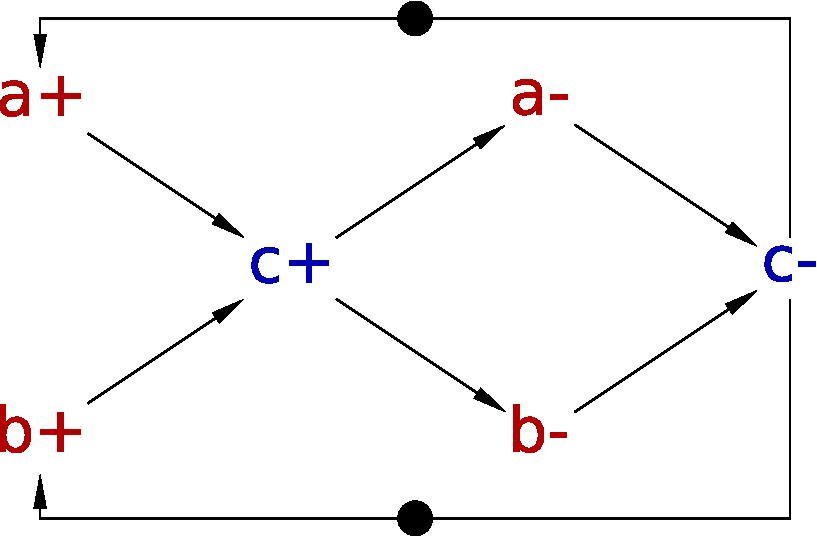
\includegraphics[scale=0.3]{Images/stg-cElement}
\par\end{centering}
\protect\caption{\label{fig:cElement STG composition}STG for the example system.}
\vspace{-4mm}
\end{figure}

Finally, the designer can also rely on protocol-level concepts, producing
the following equivalent specification:

\vspace{-3mm}
\[
\begin{array}{lcl}
\mathsf{circuit}(a,b,c)&\hspace{-2mm}=&\hspace{-2mm}\mathsf{interface}\\
~&\hspace{-2mm}\diamond&\hspace{-2mm}\mathsf{handshake00}(a,c)~\diamond~\mathsf{handshake00}(b,c)\\
\end{array}
\]

\noindent Indeed, at the high level the circuit can be seen simply as two
handshakes synchronised on a common signal.

This example demonstrates that the presented formal notation for capturing
concepts is very flexible and provides the designer with a rich selection
of available levels of abstraction, which could be used not only for
deriving simplest possible specifications but also for cross-checking
the adequacy of specifications by \emph{refactoring} them according
to the concept composition laws.

\vspace{-1mm}
\subsection{Multiple behavioural scenarios\label{sub:scenarios}}

So far we have only considered systems operating in a single behavioural
\textit{scenario} specified by a composition of concepts. However,
real-life systems often need to support multiple scenarios, e.g. start-up
and normal operation, different power modes, etc. This allows
each individual scenario to be designed using concepts,
and tested individually to ensure they work correctly, before these
are combined to produce a full system specification.

To increase the reuse of scenarios, which helps reduce design
time of future systems, this method supports the use of pre-designed
scenarios as concepts.

In some cases, a designer may find it easier to split the specification
of operational modes further than scenarios and design certain elements
separately. In this way, a model may be produced from concepts, which
may not be an operational mode on its own, but can be composed and
tested separately. Having several elements predefined
using concepts may become useful for quickly designing systems. A
predefined logic gate, for example, could be useful to quickly include
in any list of concepts when designing multiple scenarios. An STG
produced of this element can be referenced in a list of concepts by
name (provided that the definition is appropriately imported into
the current namespace). When a list of concepts is passed into the
STG translation algorithm, all referenced concepts are replaced by
the corresponding definitions.

%The process of combining scenarios is explained further in \S~\ref{sub:scenario-composition}
\vspace{-1mm}
\section{Interoperability with STG based tools\label{sec:interop-with-stg}}

Concepts are a useful way of specifying asynchronous circuits, but
specifications also need to be \emph{verified} against certain properties to ensure
their correctness, and once they are deemed to be correct, they need to
be \emph{synthesised} into efficient circuit implementations. Many software
tools exist which automatically verify and synthesise STG specifications,
such as \noun{Petrify}~\cite{Cortadella} and \noun{Mpsat}~\cite{khomenko2004detecting}.
In order to reuse the tools developed by the community, it is
necessary to be able to automatically translate concept specifications to STGs.
In this section, we present a translation algorithm~(Section~\ref{sub:translating})
and discuss ways of composing multiple behavioural scenarios into a single STG specification~(Section~\ref{sub:scenario-composition}).

\begin{algorithm}[t]
\begin{algorithmic}
\caption{Algorithm for translating concepts to STGs\label{alg:translation}}
\For {Each defined concept}
  \State \textbf{add} signal-level concepts \textbf{to} conceptList
\EndFor
%//Create consistency loops
\For {Each signal in system}
  \State \textbf{define} signal as input/output/internal
  \State \textbf{add} transition \textbf{high}
  \State \textbf{add} transition \textbf{low}
  \State \textbf{add} place \textbf{signal-0}
  \State \textbf{add} place \textbf{signal-1}
  \State \textbf{connect} (transition \textbf{high}, place \textbf{signal-1})
  \State \textbf{connect} (place \textbf{signal-1}, transition \textbf{low})
  \State \textbf{connect} (transition \textbf{low}, place \textbf{signal-0})
  \State \textbf{connect} (place \textbf{signal-0}, transition \textbf{high})
\EndFor

\For {Each causlity concept}
  \State \textbf{connect-read}(place \textbf{following} cause, effect transition)
\EndFor

\For {Each initial state concept}
  \State \textbf{add-token}(place \textbf{signal-}value)
\EndFor

\end{algorithmic}
\end{algorithm}
%A method of synthesizing concepts directly also exists, which will be explained,giving more options to designers.

\vspace{-2mm}
\subsection{Translating concepts to STGs\label{sub:translating}}

As discussed in Section~\ref{sub:Comp-of-concepts}, there are multiple ways of
representing a specification using concepts. However, all levels of
abstraction available to the designer are built out of primitive low-level
signal concepts such as causality. Given a specification, we can therefore
break down all gate- and protocol-level constructs into `atoms', which
significantly simplifies the translation task.

Using the example of a C-element with an environment, any representation
mentioned in Section~\ref{sub:Comp-of-concepts} can be broken down into the 
following list of low-level concepts:

\vspace{-3mm}
\[
\begin{array}{lcl}
\hspace{-2mm}\mathsf{circuit}(a,b,c)&\hspace{-2mm}=&\hspace{-2mm}a^{+}\rightsquigarrow c^{+} \diamond b^{+}\rightsquigarrow c^{+} \diamond c^{+}\rightsquigarrow a^{-} \diamond c^{+}
\rightsquigarrow b^{-}\\
~&\hspace{-2mm}\diamond&\hspace{-2mm}a^{-}\rightsquigarrow c^{-} \diamond b^{-}\rightsquigarrow c^{-} \diamond c^{-}\rightsquigarrow a^{+} \diamond c^{-}\rightsquigarrow b^{+}\\
~&\hspace{-2mm}\diamond&\hspace{-2mm}\mathsf{inputs}(\{a,b\})\diamond\mathsf{outputs}(\{c\})\\
~&\hspace{-2mm}\diamond&\hspace{-2mm}\mathsf{initialise}(a,0) \diamond \mathsf{initialise}(b,0)\\
~&\hspace{-2mm}\diamond&\hspace{-2mm}\mathsf{initialise}(c,0)
\end{array}
\]
%\vspace{2mm}

\noindent One can see that the above list of primitive concepts matches
the STG in Figure~\ref{fig:cElement STG composition} very closely, in particular
the causality concepts match the arcs of the STG. Below we describe a general
translation algorithm that in particular can produce this STG fully automatically.
The algorithm is implemented and integrated in the open-source tool \noun{Workcraft},
where it produces STGs in commonly used \textsf{*.g} file format.

Given a list of primitive concepts, the algorithm starts by creating so-called
\emph{consistency loops} for each signal in the specified interface, which forces rising
and falling transitions of each signal to alternate, thereby ensuring that the resulting
STG satisfies the property of \emph{consistency}~\cite{Cortadella}.
The places between the transitions of a signal determine its state.
Figure~\ref{fig:step-by-step1} shows consistency loops created for the example.
\vspace{-2mm}
\begin{figure}[h]
\begin{centering}
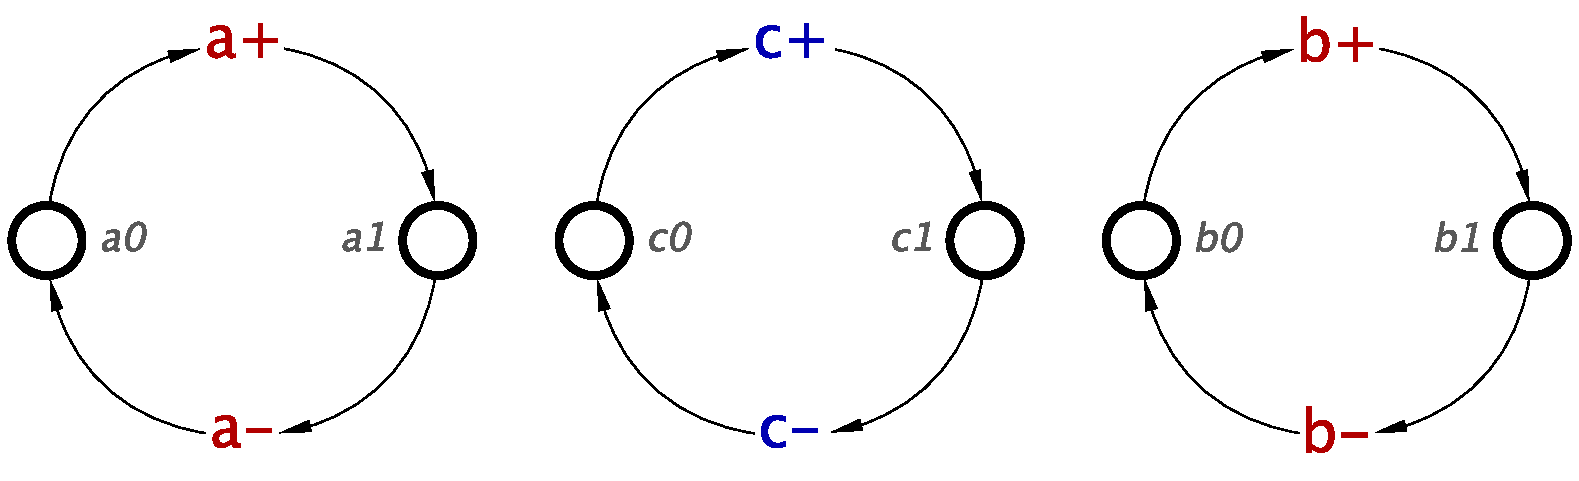
\includegraphics[scale=0.3]{Images/Step-by-step1}
\par
\protect\caption{\label{fig:step-by-step1}The first step: create consistency loops.}
\vspace{-2mm}
\end{centering}
\end{figure}

The next step is to connect signal transitions according to the list of causality
concepts. In the above example we start with $a^{+}\rightsquigarrow c^{+}$.
To represent it in the STG, we connect the place after $a^{+}$ ($a1$ in
Figure~\ref{fig:step-by-step1}) to transition $c^{+}$ by a \emph{read arc},
which allows $c^{+}$ to transition without consuming the token (consuming
the token would disable $a^{-}$), see Figure~\ref{fig:step-by-step2}.

\vspace{-2mm}
\begin{figure}[h]
\begin{centering}
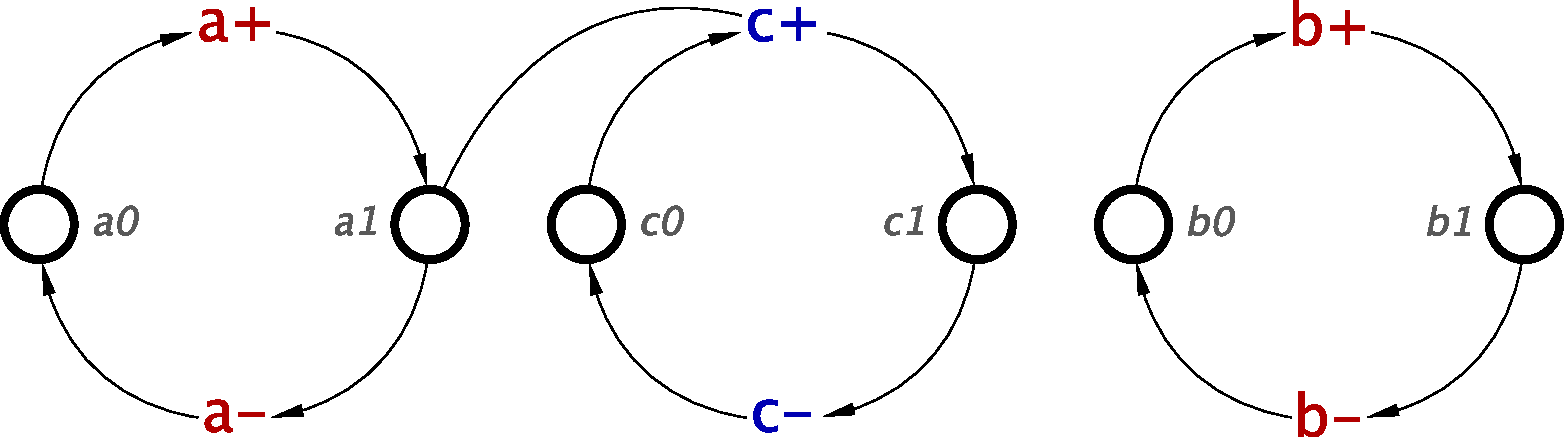
\includegraphics[scale=0.3]{Images/Step-by-step2}
\par
\protect\caption{\label{fig:step-by-step2}The second step: add causality concept $a^{+}\rightsquigarrow c^{+}$.}
\vspace{-2mm}
\end{centering}
\end{figure}

We continue translating the remaining causality concepts in the same manner
obtaining the STG shown in Figure~\ref{fig:step-by-step9}.

\vspace{-2mm}
\begin{figure}[h]
\begin{centering}
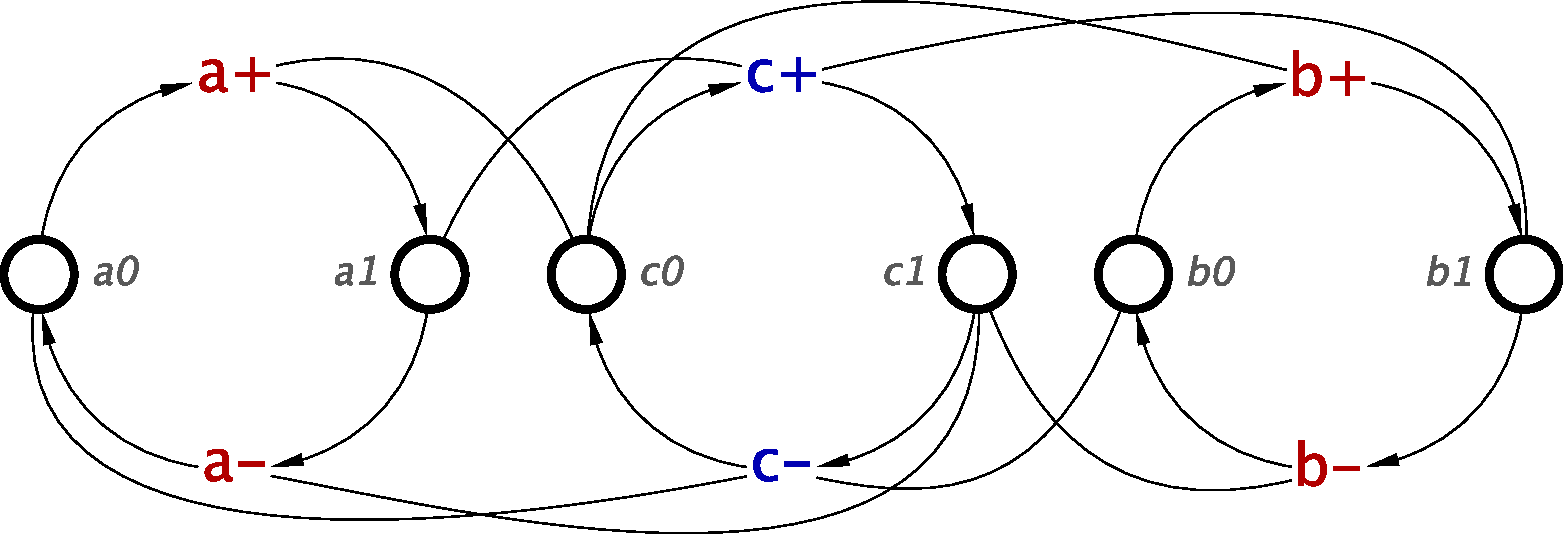
\includegraphics[scale=0.3]{Images/Step-by-step9}
\par
\protect\caption{\label{fig:step-by-step9}Finish the second step: add all causality concepts.}
\vspace{-2mm}
\par\end{centering}
\end{figure}

The final step of the translation algorithm is to add tokens to some of the places
of the resulting STG according to the initial state concepts
$\mathsf{initialise}(a,0) \diamond \mathsf{initialise}(b,0) \diamond \mathsf{initialise}(c,0)$, which declare the initial states of all three signals to be 0. We therefore
add tokens to places $a0$, $b0$ and $c0$, producing the fully translated STG in
Figure~\ref{fig:step-by-step12}.

\begin{figure}[h]
\begin{centering}
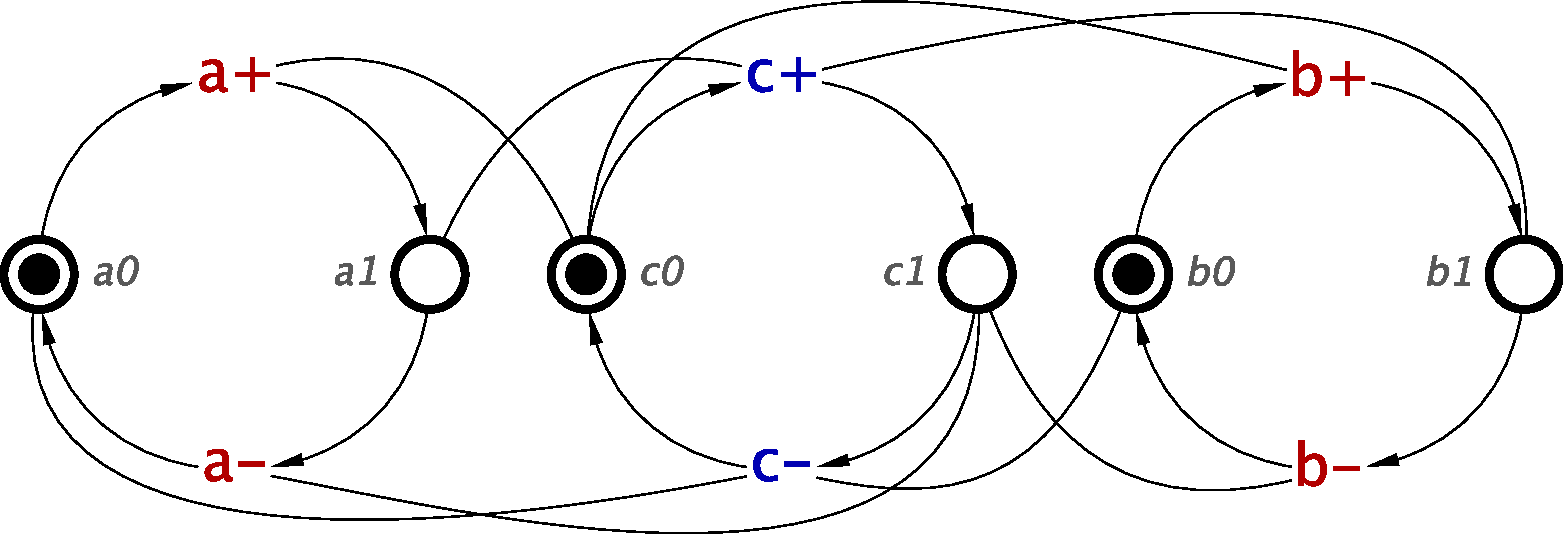
\includegraphics[scale=0.3]{Images/Step-by-step12}
\par
\protect\caption{\label{fig:step-by-step12}The final step: set the initial state.}
\par\end{centering}
\vspace{-3mm}
\end{figure}

The resulting STG and the STG shown in Figure~\ref{fig:cElement STG composition}
look very different but they are behaviourally equivalent. The latter is much more
compact and easier to read though, and it would be preferable to show it to the
designer instead of the one obtained by our translation algorithm. Our
implementation supports automated \emph{resynthesis} of the resulting STG
using \noun{Petrify}, and can therefore seamlessly produce the STG in
Figure~\ref{fig:cElement STG composition} from the given specification.

%By integrating concepts into \noun{Workcraft} we allow a designer to
%visualise their concept designs as STGs, to simulate, verify and synthesise them,
%and if there are any corrections or additions to be made these can be done either
%directly in the STG or in the original concept specification, which can then
%be re-translated into an updated STG.

%In some cases it may not be necessary to visualize a translated STG. A \emph{.g} file is used as an input with these tools, without having to import into \noun{Workcraft}. This can
%further quicken the process of specification using concepts. This also applies to synthesis, which can be performed using a tool such as \noun{Petrify} or \noun{Mpsat}.

%or using \emph{Direct Synthesis}, which is discussed in \S\ref{sub:direct-synth}.

The described translation algorithm is shown in pseudocode
in~Algorithm~\ref{alg:translation}.

\vspace{-1mm}
\subsection{Partial translation and parallel composition}

In some cases it may be useful to partially translate concepts to STGs, for
example to investigate the behaviour of a circuit
in different environments. An important property of the above algorithm is
that it can be applied to incomplete systems, thereby translating
smaller collections of concepts, or even singular concepts, which do not
necessarily correspond to well-behaving STGs (e.g. the resulting STGs may contain
spurious input transitions if they are not controlled by the environment).
Such partial specifications can be visualised, studied, and then composed into
complete specifications using the \emph{parallel composition}, which is supported
by \noun{Workcraft} using an integrated tool \noun{Pcomp}~\cite{PCOMP}.

\begin{figure}[t]
\begin{centering}
\subfloat[\label{fig:cElement}$\mathsf{cElement}(a,b,c)$]{\begin{centering}
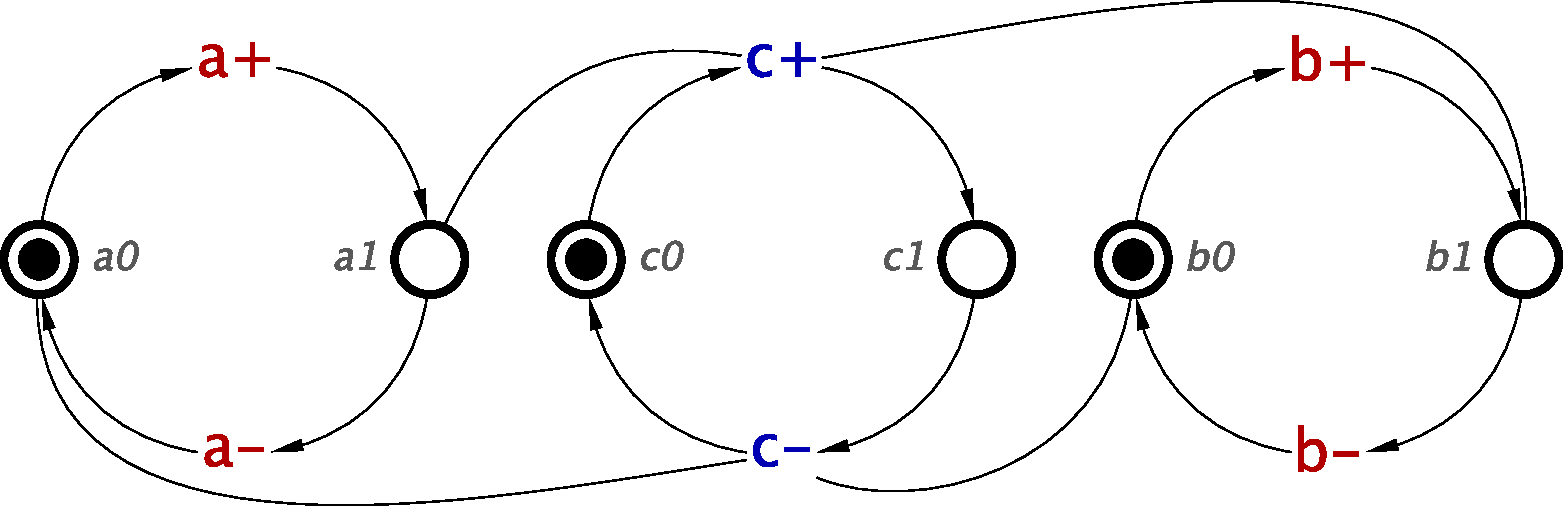
\includegraphics[scale=0.3]{Images/C-element}
\par\end{centering}
}
\par
\subfloat[\label{fig:inverterca}$\mathsf{inverter}(c,a)$]{\begin{centering}
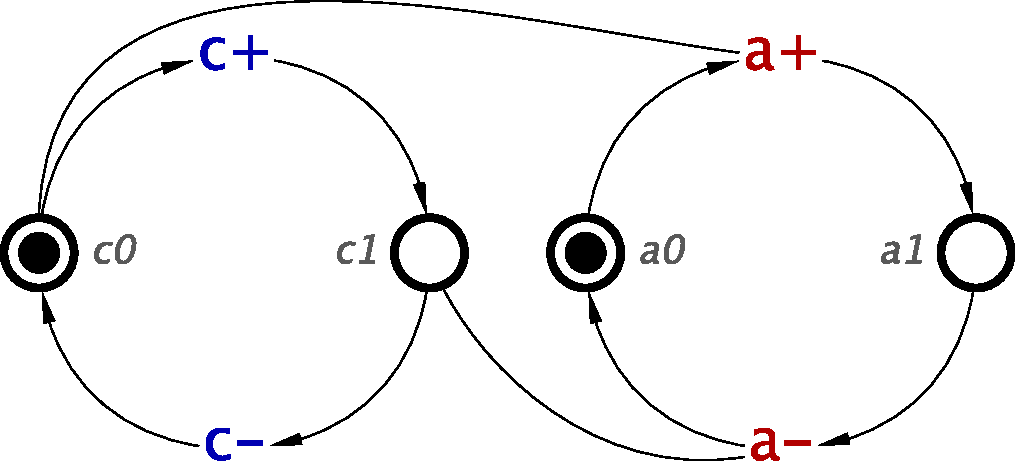
\includegraphics[scale=0.3]{Images/inverter(c,a)}
\par\end{centering}

}
\par
\subfloat[\label{fig:inverterba} $\mathsf{inverter}(c,b)$]{\begin{centering}
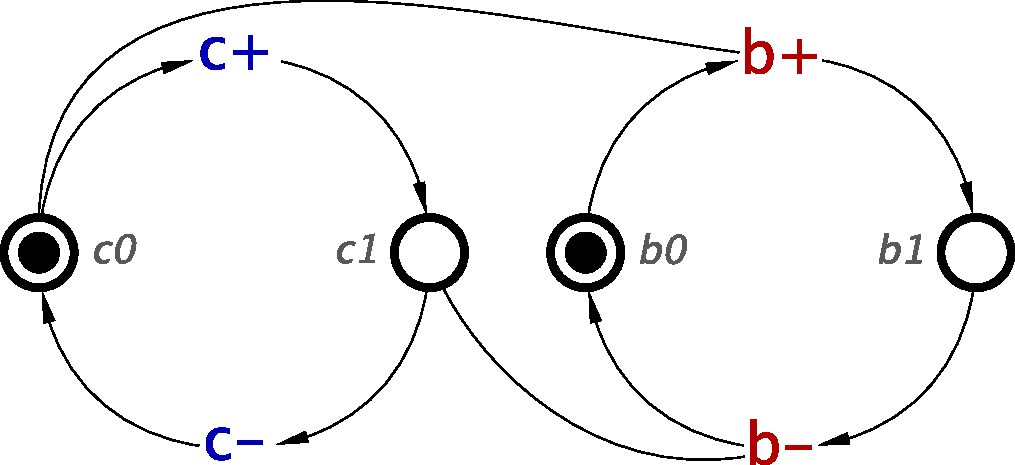
\includegraphics[scale=0.3]{Images/inverter(c,b)}
\par\end{centering}
}
\par\end{centering}
\protect\caption{\label{fig:IndividConceptStgs}Partial translation of concepts into STGs}
\vspace{-6mm}
\end{figure}

Using the example in Section~\ref{sub:Comp-of-concepts}, a C-element with environment,
we can translate the concepts corresponding to the C-element and the two
environment inverters individually. Including the initial states, this would
give us the STGs found in Figure~\ref{fig:IndividConceptStgs}. These STGs can be
composed using the parallel composition, the outcome of which will be equivalent
to the result obtained by translating the complete specification, bringing us back
to the STG in Figure~\ref{fig:cElement STG composition}.

\vspace{-1mm}
\subsection{Scenario combination\label{sub:scenario-composition}}

As mentioned in Section~\ref{sub:scenarios}, concepts are used to specify
a single behavioural scenario.
%which can be tested and verified separately to allow for easier changes and additions
%to smaller, less complex, specifications. However, when scenarios are tested and prove to work as required, and satisfy all necessary properties, they then need to be combined to
%produce a full system specification, so this can be tested and verified, and ultimately be synthesized to produce an implementation.
When combining scenarios, there are several things to consider in
how the scenarios fit together. Depending on the application,
%the circuit is being designed for
some scenarios may need to operate in certain
orders, for example, one scenario may exist simply to initialise the
circuit, therefore this scenario needs to run at start-up, before
any other scenario, and then never be run again while the
system remains active.

To address this, we can define \emph{templates},
which can be used to combine scenarios in various ways.
With this the designer specifies how the scenarios should
be combined, and if an order is needed, the order the scenarios should
be run from start up. The following are some examples of templates
that can be used to combine scenarios:

\textbf{Sequential template:} Sequential combination will allow a designer
to select the order of all scenarios, so when combined, they will
run in a sequence. In this case, there may be a clear order in which
the scenarios may run, and this needs to be specified by the designer:

%\vspace{-2mm}
\begin{center}
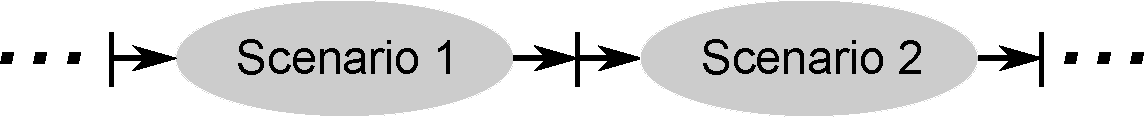
\includegraphics[scale=0.42]{Images/sequential_combination}
\end{center}

\textbf{Concurrent template:} In this case there is no order, but one or more
of the scenarios in a specification may run concurrently. It may be necessary
to limit concurrency by specifying, for instance, the number of scenarios
that can be active simultaneously:

\vspace{-2mm}
\begin{center}
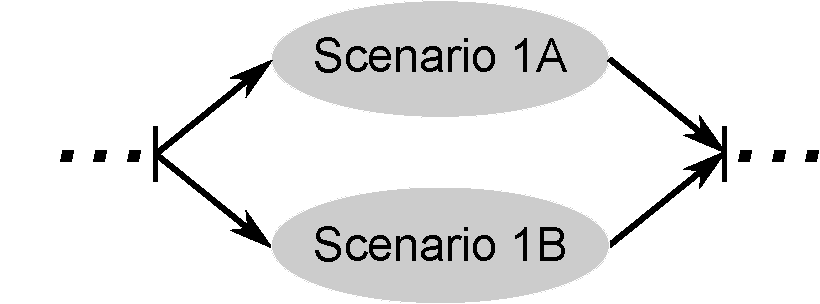
\includegraphics[scale=0.42]{Images/concurrent_combination}
\end{center}

\textbf{Non-deterministic choice template:} This template will combine the
scenarios in a way that allows any of the scenarios to run, but not
according to any order to deal with the lack of determinism in the
system, using one token which is used only by the running scenario,
and returned when the scenario completes:

\vspace{2mm}
\begin{center}
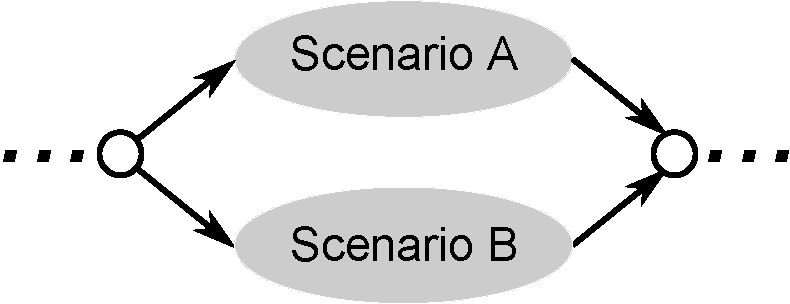
\includegraphics[scale=0.42]{Images/non_deterministic_combination}
\end{center}

There may be more complex requirements to combination of scenarios, and it
is possible to combine some scenarios using one template, then including
the result in a combination with other scenarios using another template.
For example, a system which is non-deterministic may also have a scenario
that runs at start up. In this case, a designer could combine all
non-deterministic scenarios first, then combine the resulting STG with
the initialising scenario, setting the order so this runs first.

This method can allow for many possible scenario combination
styles, and more complex systems can be combined automatically, which
in comparison to manual combination, could reduce the number of errors
as well as design time.

\subsection{Tool integration}

The concepts tool, which translates asynchronous concepts to STGs has been
integrated into open-source toolsuite \noun{Workcraft}~\cite{Workcraft_website}.
This allows a designer to visualise their concept designs as STGs, to simulate,
verify and synthesise them using other tools integrated in \noun{Workcraft},
and if there are any corrections or additions to be made these can be done either
directly in the STG or in the original concept specification, which can then
be re-translated into an updated STG. These automated processes can allow for a streamlined design process of asynchronous circuits.

Scenario combination is not yet implemented and is performed manually by
the designer using \noun{Workcraft}'s graphical user interface. This
design stage can also be automated to further streamline the design process
using concepts.

\vspace{-1mm}
\section{Case study\label{sec:case-study}}

In Section~\ref{sec:Motivating Example} we introduced the motivating example for
this article, a simple buck converter, and discussed the challenges of monolithic
approach to specifying asynchronous circuits. We have also introduced
concepts in Section~\ref{sec:Concepts}, and with examples explained how they can
be used to design simple circuits, and how these can be translated to STGs
for subsequent synthesis of asynchronous gate-level implementation.
In this section we use the buck converter as a case study to detail the
whole design process in \noun{Workcraft}, see Figure~\ref{fig:workcraft_screenshot}.

%\vspace{-5mm}
\begin{figure*}[t]
\begin{centering}
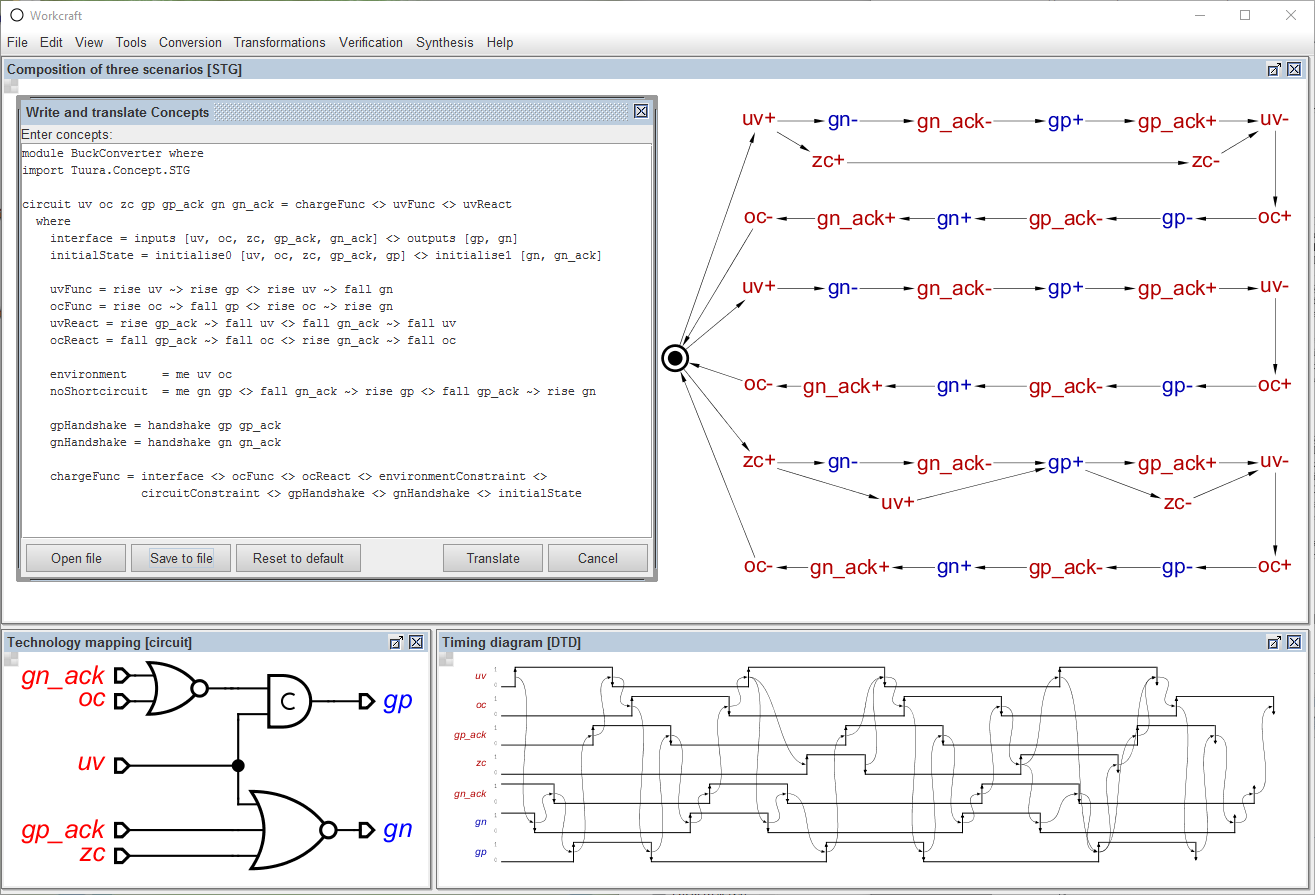
\includegraphics[scale=0.5]{Images/design_flow_wc_screenshot}
\par\end{centering}

\protect\caption{\label{fig:workcraft_screenshot}Stages of the design flow when using asynchronous concepts in \noun{Workcraft}.}
\vspace{-4mm}
\end{figure*}

\subsection{Formal specification using concepts}

The informal specification of the buck converter defines three operating modes
that require distinctive control scenarios. Requirements for each operating mode
can be captured with a separate list of concepts and translated into scenario
STGs. These can be subsequently combined to produce single STG for the whole circuit.
During this process, it is useful to find any operations which occur
between two or more operating modes, as these can then be reused.

\subsubsection{ZC~absent scenario}

A circuit that handles buck operation in absence of ZC condition is specified as follows:

%\vspace{-4mm}
\newpage
\[
\mathsf{zcAbsentScenario}(uv,oc,zc,gp,gp\_ack,gn,gn\_ack)~~~~~~~~~~~~~~~~~~~~~~~~~~~~~~~
\]
\vspace{-6mm}
\[
~~=~\mathsf{chargeFunc}~\diamond~\mathsf{uvFunc}~\diamond~\mathsf{uvReact}
\]
\vspace{-5mm}
\[
\begin{array}{lcl}
\mathsf{where}&~&\\

~~~~\mathsf{interface}&\hspace{-2mm}=&\hspace{-2mm}\mathsf{inputs}~[uv, oc, zc, gp\_ack, gn\_ack]\\
~&\hspace{-2mm}\diamond&\hspace{-2mm}\mathsf{outputs}~[gp, gn]\\

~~~~\mathsf{uvFunc}&\hspace{-2mm}=&\hspace{-2mm}uv^{+}\rightsquigarrow gp^{+}~\diamond~ uv^{+}\rightsquigarrow gn^{-}\\

~~~~\mathsf{ocFunc}&\hspace{-2mm}=&\hspace{-2mm}oc^{+}\rightsquigarrow gp^{-}~\diamond~ oc^{+}\rightsquigarrow gn^{+}\\

~~~~\mathsf{uvReact}&\hspace{-2mm}=&\hspace{-2mm}gp\_ack^{+}\rightsquigarrow uv^{-}~\diamond~gn\_ack^{-}\rightsquigarrow uv^{-}\\

~~~~\mathsf{ocReact}&\hspace{-2mm}=&\hspace{-2mm}gp\_ack^{-}\rightsquigarrow oc^{-}~\diamond~gn\_ack^{+}\rightsquigarrow oc^{-}\\

~~~~\mathsf{environment}&\hspace{-2mm}=&\hspace{-2mm}\mathsf{me}(uv, oc)\\

~~~~\mathsf{\mathsf{noShortcircuit}}&\hspace{-2mm}=&\hspace{-2mm}\mathsf{me}(gn, gp)\\
~&\hspace{-2mm}\diamond&\hspace{-2mm}gn\_ack^{-}\rightsquigarrow gp^{+}~\diamond~gp\_ack^{-}\rightsquigarrow gn^{+}\\

~~~~\mathsf{gpHandshake}&\hspace{-2mm}=&\hspace{-2mm}\mathsf{handshake}(gp,gp\_ack)\\

~~~~\mathsf{gnHandshake}&\hspace{-2mm}=&\hspace{-2mm}\mathsf{handshake}(gn,gn\_ack)\\

~~~~\mathsf{initialState}&\hspace{-2mm}=&\hspace{-2mm}\mathsf{initialise0}~[uv,oc,zc,gp,gp\_ack]\\
~&\hspace{-2mm}\diamond&\hspace{-2mm}\mathsf{initialise1}~[gn,gn\_ack]\\

~~~~\mathsf{chargeFunc}&\hspace{-2mm}=&\hspace{-2mm}\mathsf{interface}~\diamond~\mathsf{ocFunc}~\diamond~\mathsf{ocReact}\\
~&\hspace{-2mm}\diamond&\hspace{-2mm}\mathsf{environment}~\diamond~\mathsf{noShortcircuit}\\
~&\hspace{-2mm}\diamond&\hspace{-2mm}\mathsf{gpHandshake}~\diamond~\mathsf{gnHandshake}\\
~&\hspace{-2mm}\diamond&\hspace{-2mm}\mathsf{initialState}

\end{array}
\]

The \textsf{zcAbsentScenario} concept is a composition of buck charging and UV handling.
Consider the charging function captured in \textsf{chargeFunc} concept.
It comprises several concepts: \textsf{interface} specifies the types
of signals and \textsf{initialState} defines their initial state;
\textsf{gpHandshake} and \textsf{gnHandshake} specify the protocol on $gp/gp\_ack$
and $gn/gn\_ack$ interfaces respectively;
\textsf{noShortcircuit} enforces a safety constraint to prevent a shortcircuit;
\textsf{ocFunc} and \textsf{ocReact} define the interplay with OC condition;
and \textsf{environment} captures the fact that OC and UV conditions never happen at the same time.

Note that the sequence of PMOS/NMOS switching during the charging cycle is the same
for all operating modes, and therefore the \textsf{chargeFunc} concept can be reused
in other scenarios.

\begin{figure}[H]
\vspace{-3mm}
\begin{centering}
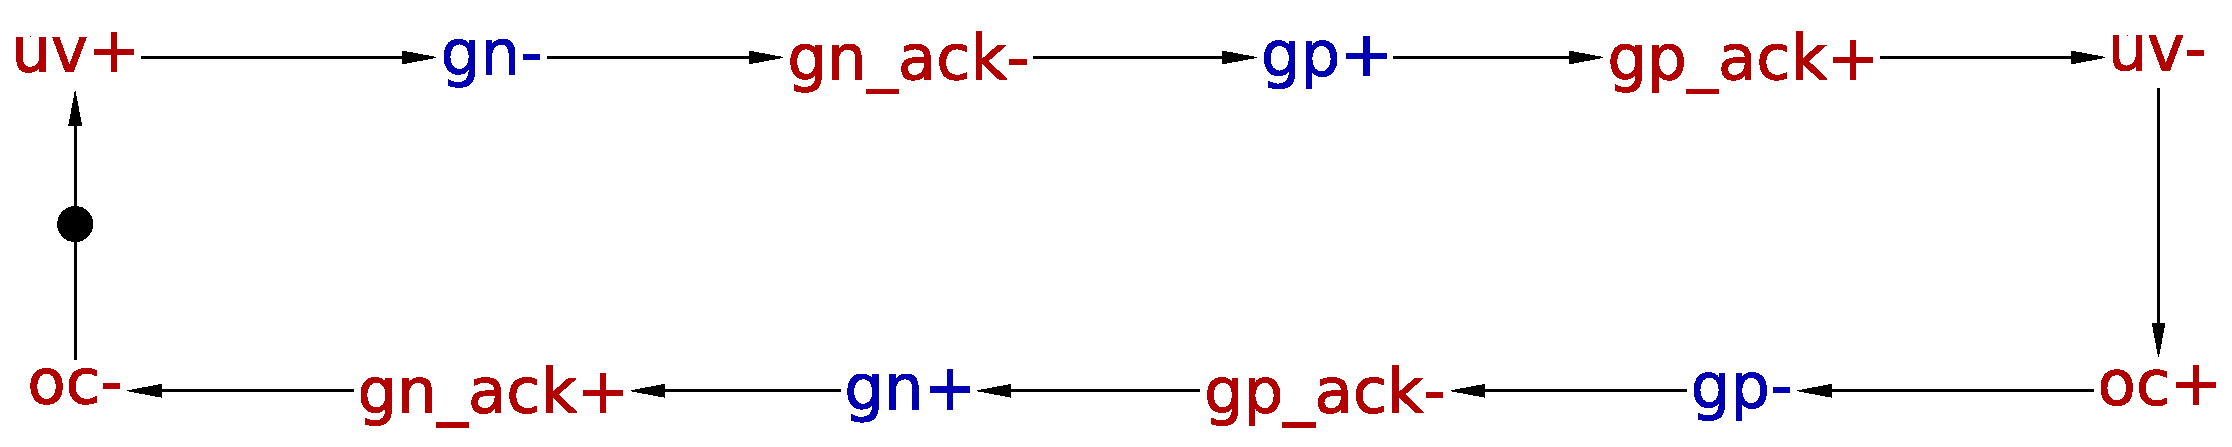
\includegraphics[scale=0.23]{Images/stg-UV_without_ZC}
\par\end{centering}
\protect\caption{\label{fig:zcAbsentScenario STG} STG for the \textsf{zcAbsentScenario} concept.}
\end{figure}

The \textsf{zcAbsentScenario} concept is automatically translated to the STG specification
in Figure~\ref{fig:zcAbsentScenario STG}.

\subsubsection{ZC~late scenario}


If ZC condition is detected after UV, then buck operation is the same as in
absence of ZC, i.e. ZC conditions can be ignored. This is captured by an additional
\textsf{zcLate} concept:

\vspace{-4mm}
\[
\mathsf{zcLateScenario}(uv,oc,zc,gp,gp\_ack,gn,gn\_ack)~~~~~~~~~~~~~~~~~~~~~~~~~~~~~~~
\]
\vspace{-6mm}
\[
~~=~\mathsf{chargeFunc}~\diamond~\mathsf{uvFunc}~\diamond~\mathsf{uvReact}~\diamond~\mathsf{zcLate}
\]
\vspace{-5mm}
\[
\begin{array}{lcl}
\mathsf{where}&~&\\

~~~~\mathsf{zcLate}&\hspace{-2mm}=&\hspace{-2mm}uv^{+}\rightsquigarrow zc^{+}~\diamond~ zc^{-}\rightsquigarrow uv^{-}~~~~~~~~~~~~~~~~~~~~~~~~~~~

\end{array}
\]

The STG specification automatically produced from the \textsf{zcLateScenario} concept
is shown in Figure~\ref{fig:zcLateScenario STG}. It looks similar to the STG in
Figure~\ref{fig:zcAbsentScenario STG} but features a concurrent branch for $zc$ signal.
Note that the arc $zc^{+}\rightsquigarrow zc^{-}$ is implied at translation
time by consistency loops.

\begin{figure}[H]
\begin{centering}
\vspace{-1mm}
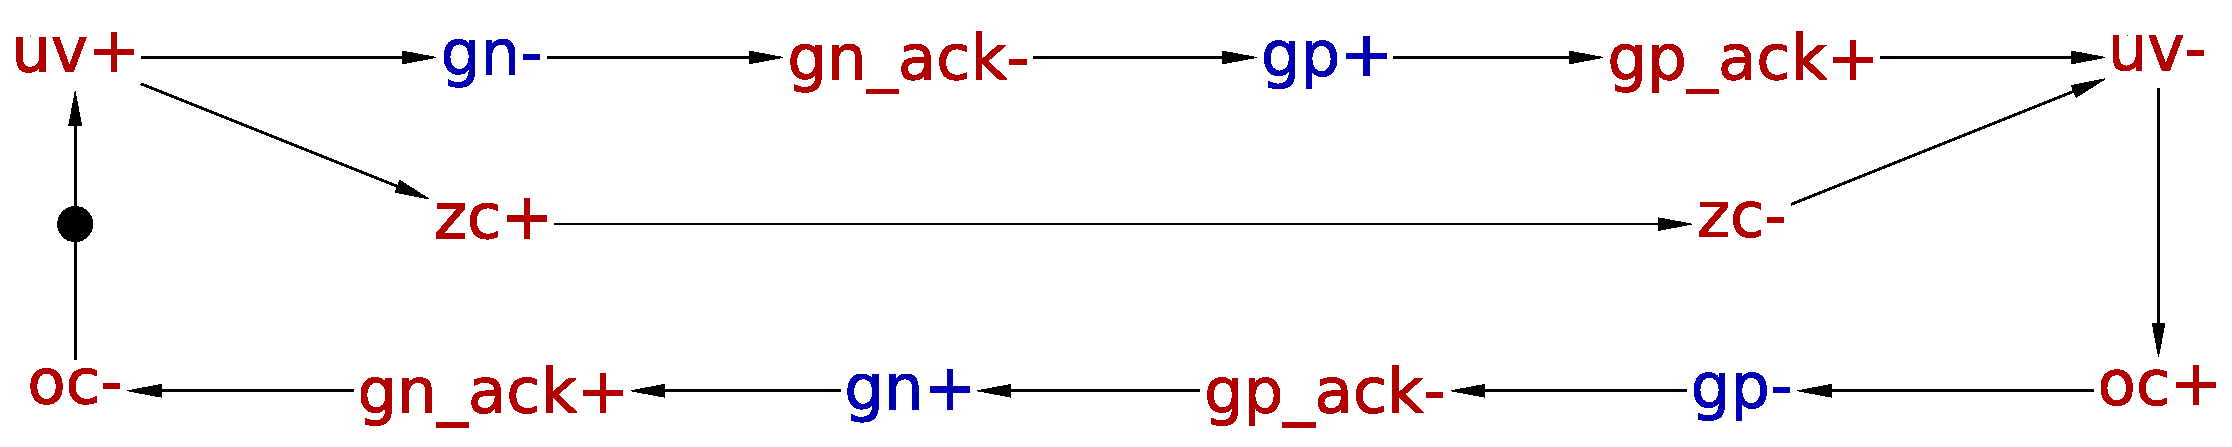
\includegraphics[scale=0.23]{Images/stg-UV_before_ZC}
\par\end{centering}
\vspace{-1mm}
\protect\caption{\label{fig:zcLateScenario STG}STG for the \textsf{zcLateScenario} concept.}
\vspace{-3mm}
\end{figure}

Note that the concept specification of \textsf{zcLateScenario} reuses most of
the code from the \textsf{zcAbsentScenario}; in particular, the description of
the analogue environment does not need to be duplicated, as with the STG
approach, where the designer needs to redraw the specification from scratch.
\noun{Workcraft} allows to copy and paste STGs, which mitigates the problem
somewhat, but duplication and associated design problems remain -- for example, if
the analogue environment needs to be amended, these changes need to be done
consistently in all scenarios. With concepts, only one definition needs to be
changed, which increases the productivity of the designer.

\subsubsection{ZC~early scenario}

If ZC condition is detected before UV then it needs to be explicitly
handled by the control circuit:

\vspace{-4mm}
\[
\mathsf{zcEarlyScenario}(uv,oc,zc,gp,gp\_ack,gn,gn\_ack)~~~~~~~~~~~~~~~~~~~~~~~~~~~~~~~
\]
\vspace{-5mm}
\[
\begin{array}{lcl}
~~=~\mathsf{chargeFunc}~\diamond~\mathsf{zcFunc}~\diamond~\mathsf{zcReact}~\diamond~\mathsf{uvFunc'}\\
~~~\!\diamond~~~~\!\!\mathsf{uvReact'}\\
\end{array}
\]
\vspace{-4mm}
\[
\begin{array}{lcl}
\mathsf{where}&~&\\

~~~~\mathsf{zcFunc}&\hspace{-2mm}=&\hspace{-2mm}zc^{+}\rightsquigarrow gn^{-}\\
~~~~\mathsf{zcReact}&\hspace{-2mm}=&\hspace{-2mm}oc^{-}\rightsquigarrow zc^{+}~\diamond~gp^{+}\rightsquigarrow zc^{-}\\
~~~~\mathsf{uvFunc'}&\hspace{-2mm}=&\hspace{-2mm}uv^{+}\rightsquigarrow gp^{+}\\
~~~~\mathsf{uvReact'}&\hspace{-2mm}=&\hspace{-2mm}zc^{+}\rightsquigarrow uv^{+}
\diamond~zc^{-}\rightsquigarrow uv^{-}\\
&\hspace{-2mm}\diamond&\hspace{-2mm}gp\_ack^{+}\rightsquigarrow uv^{-}

\end{array}
\]

The obtained STG for the \textsf{zcEarlyScenario} concept is shown
in Figure~\ref{fig:zcEarlyScenario STG}.

\begin{figure}[H]
\begin{centering}
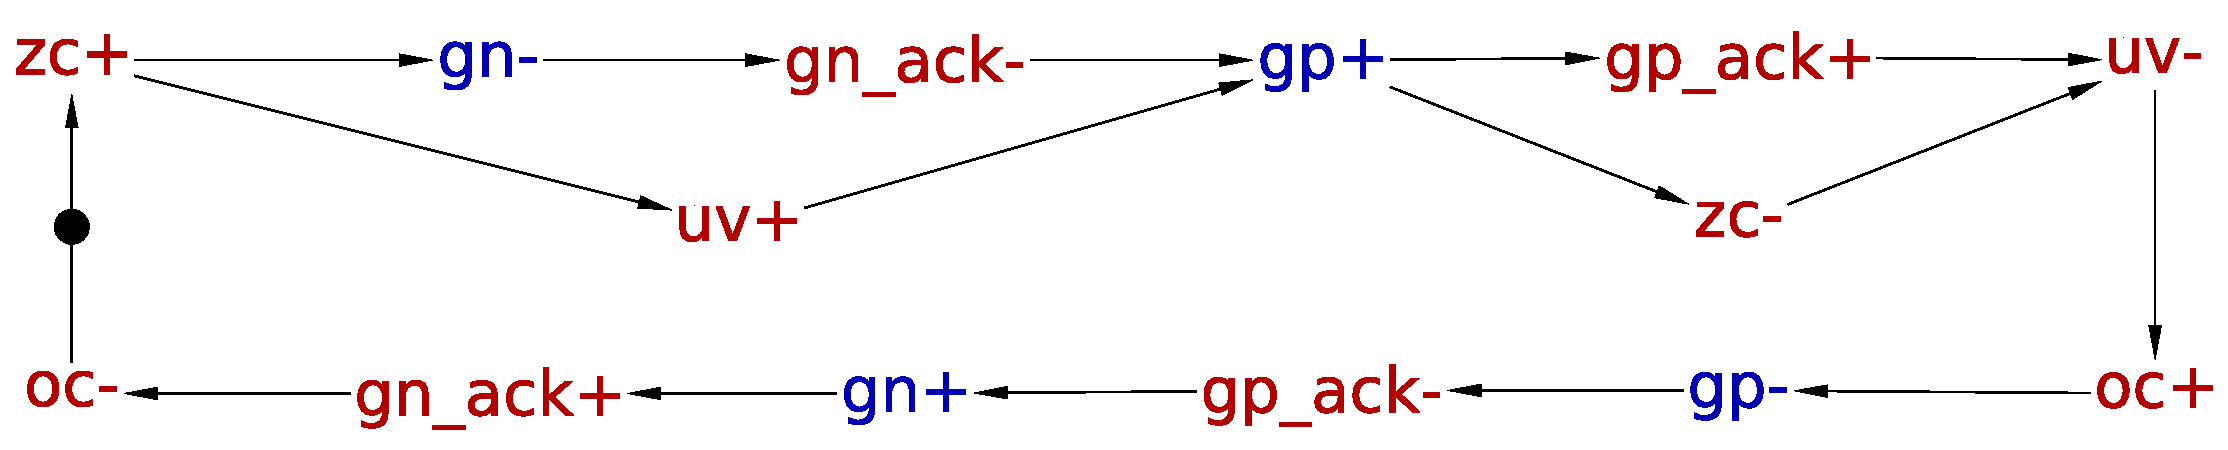
\includegraphics[scale=0.23]{Images/stg-UV_after_ZC}
\par\end{centering}
\protect\caption{\label{fig:zcEarlyScenario STG}STG for the \textsf{zcEarlyScenario} concept.}
\vspace{-3mm}
\end{figure}

\subsection{Combining the scenarios }

The scenario STGs can now be combined as described in Section~\ref{sub:scenario-composition}
to produce a multi-scenario specification. As buck operating modes are active one at a
time, the control scenarios are combined using the non-deterministic choice template.

Figure~\ref{fig:buck STG} shows the resulting STG specification. This can be
further simplified by merging the common parts of the scenarios, thus producing
a more compact model similar to that shown in Figure~\ref{fig:Monolithic-buck}.

There is an explicit place in this model which holds a token initially
and allows any of the scenarios to run. This free-choice place has no
control over which scenario can run, and only allows one of
them to run at a time.

%\vspace{-3mm}

\subsection{Verification and simulation}

To be combinable by our method, the scenario STGs need to satisfy certain
properties~\cite{Cortadella}:
\begin{itemize}
\item Complete State Coding (CSC): each state of the models with different
behaviour has differing signal encodings to avoid problems during
synthesis. Note that in most cases it is possible to automatically
resolve CSC conflicts.
\item Deadlock freedom: no state is reachable from which no progress can
be made.
\item Output persistence: there are no race conditions in the STG (i.e. no glitches).
\item Signal consistency: in any trace the rising and falling transitions of
each signal alternate.
\end{itemize}
These properties can be automatically checked in \noun{Workcraft} using
the \noun{Mpsat}~\cite{khomenko2004detecting} backend tool.
It is also possible to verify custom safety properties expressed using
syntax similar to SystemVerilog Assertions, which is familiar to many
hardware designers.
Figure~\ref{fig:custom_assertion} contains an example custom assertion
\textsf{!($gp$ \&\& $gn$)} that we created for this case study.
In this we formally verify that there is no shortcircuit in the system, by
checking that $gp$ and $gn$ are never high at the same time.
As seen in this image, the property correctly holds, as expected.

\begin{figure}[t]
\begin{centering}
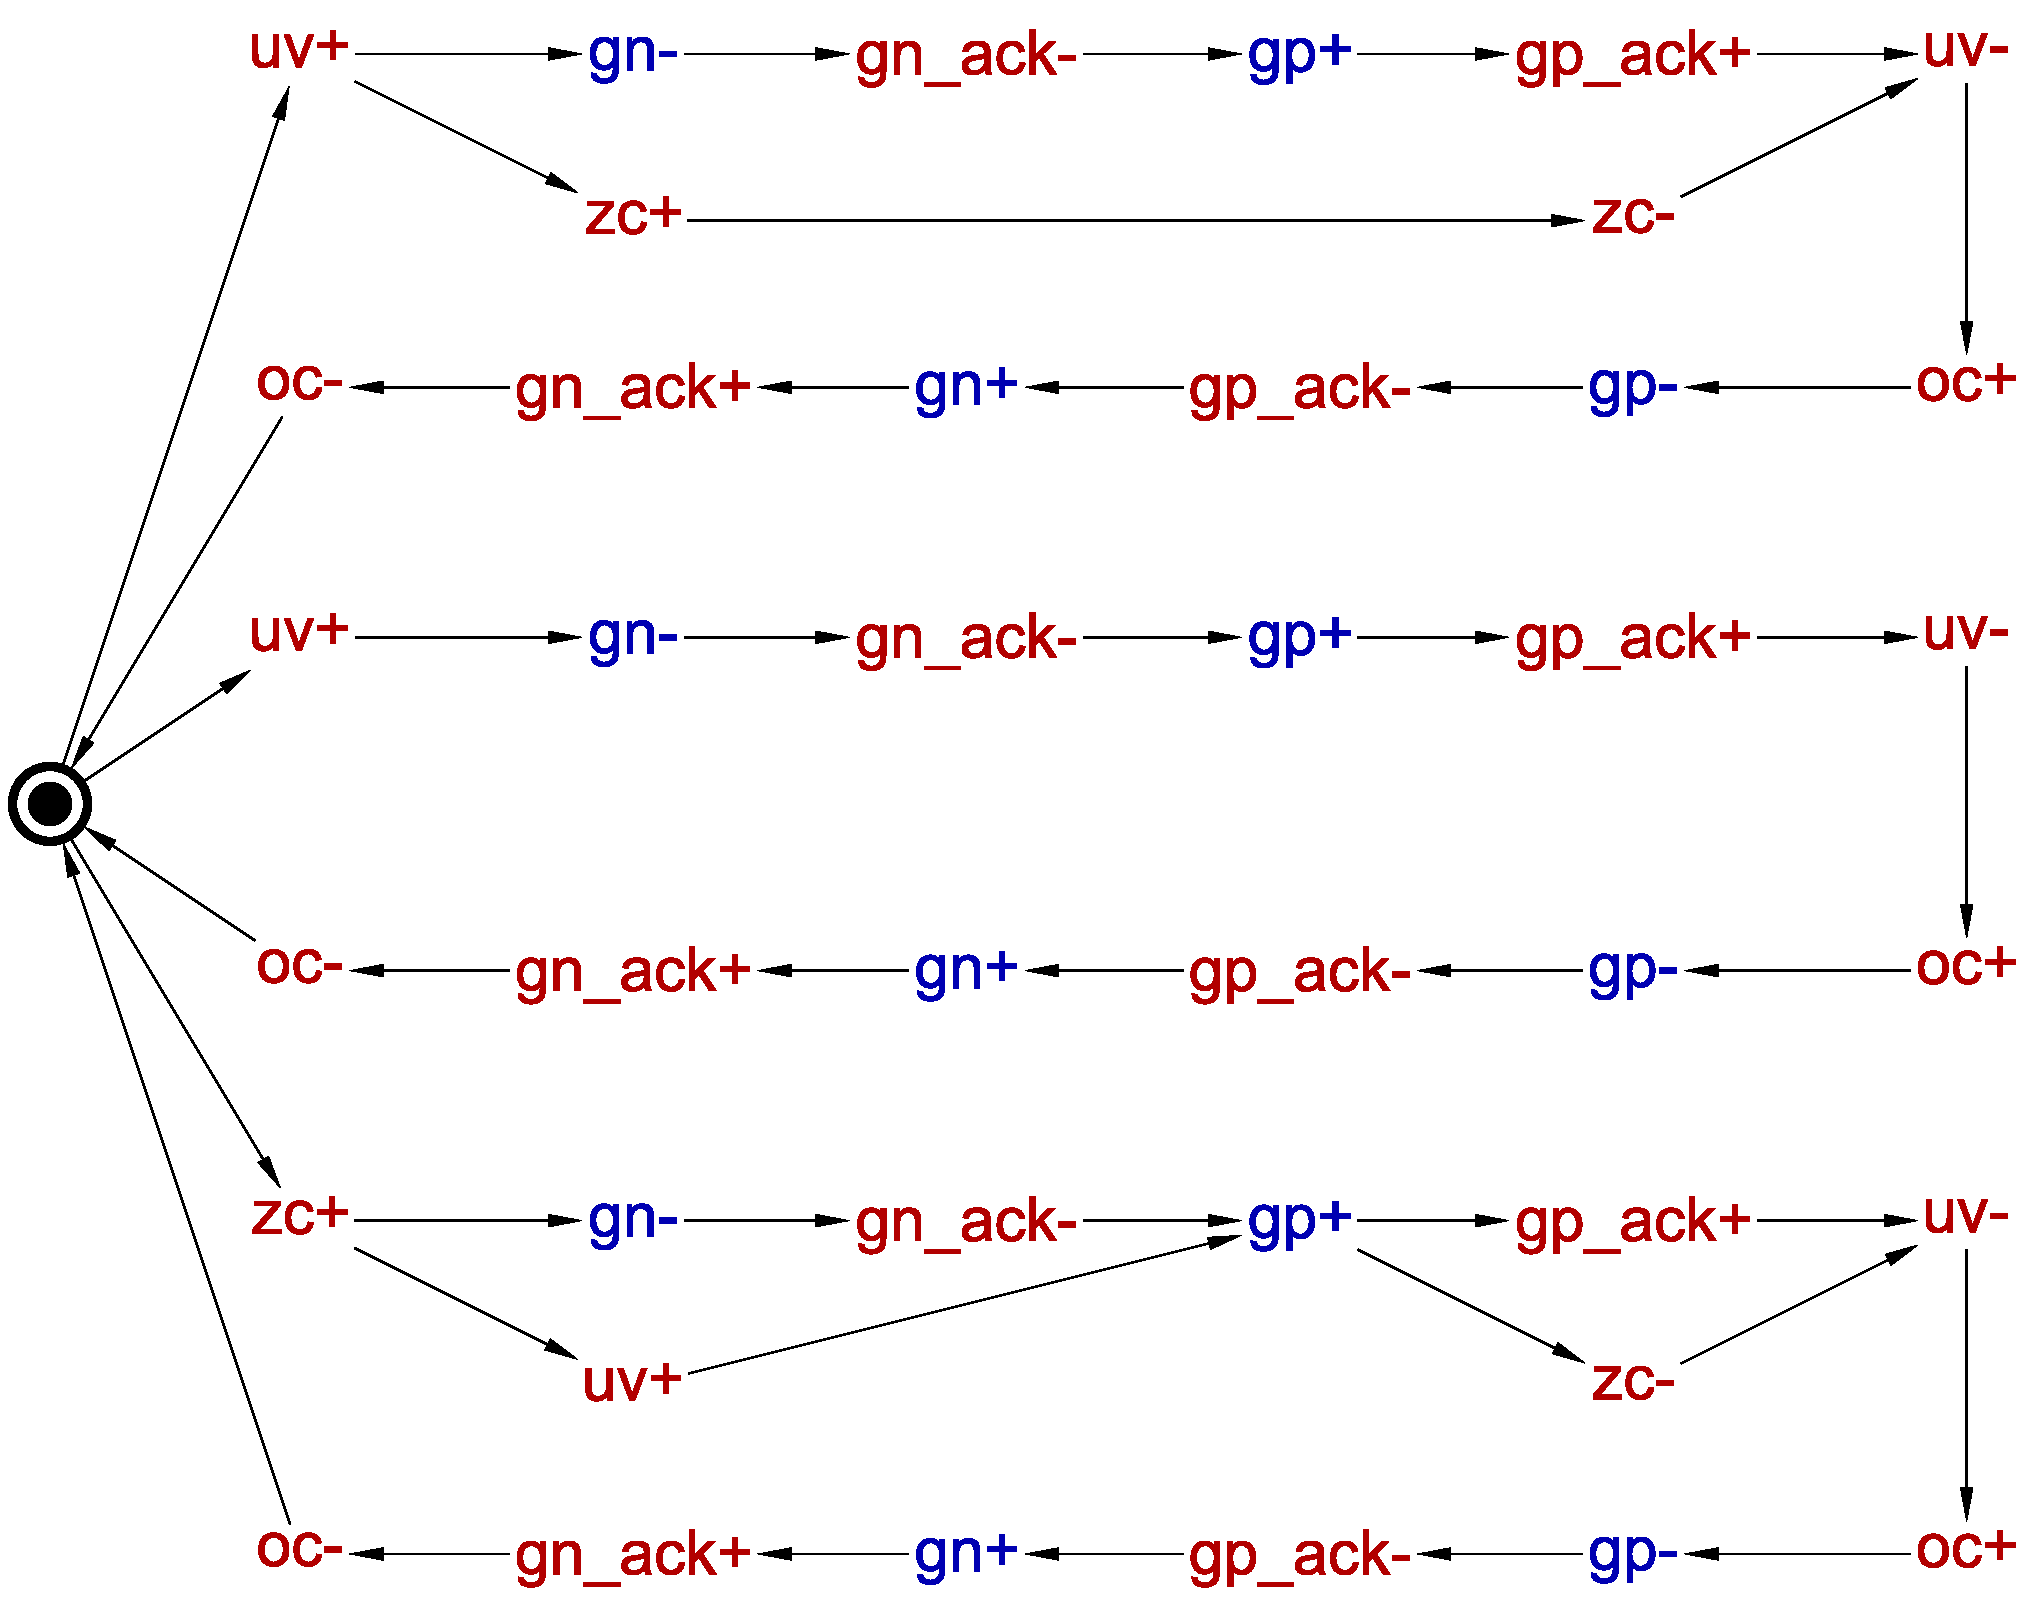
\includegraphics[scale=0.23]{Images/stg-buck-scenarios_merged}
\par\end{centering}
\begin{centering}
\protect\caption{\label{fig:buck STG}Complete STG for a buck converter.}
\par\end{centering}
\vspace{-3mm}
\end{figure}

\begin{figure}[h]
\begin{centering}
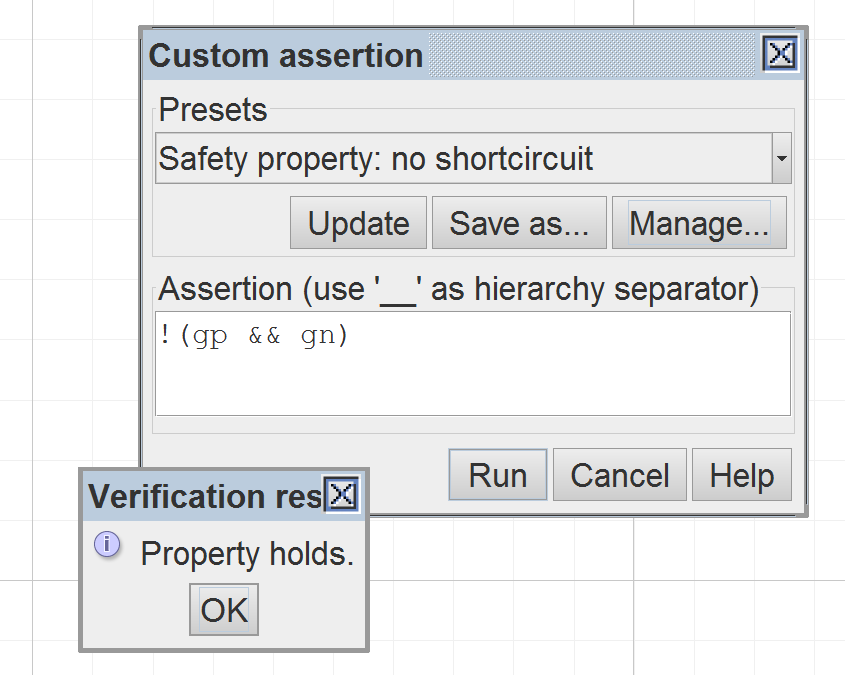
\includegraphics[scale=0.75]{Images/screenshot-custom-assertion}
\par\end{centering}
\begin{centering}
\protect\caption{\label{fig:custom_assertion}Custom verification of no shortcircuit.}
\par\end{centering}
\vspace{-3mm}
\end{figure}

In the event that one of these properties does not hold, unless it can be corrected
automatically, which \noun{Mpsat} can attempt, the combination of scenarios fails.
In this case a problematic concept can be identified and diagnostic information
is printed out to help a designer correct the issue.

Correctly produced scenarios may not necessarily work as the designer expects,
and this needs to be validated before using these scenarios
in any further designs. In addition to formal verification, \noun{Workcraft}
features a simulation tool,
and this can be used by a designer to check that the signals can transition
according to the initial requirements. If the simulation produces
undesirable results, a designer can work to fix the error of the scenario
STG, or correct the design at the concept level. The latter is the
preferable method if the design is to be reused either as a predefined
concept, or as a scenario in another system.

After all scenarios have been combined, the result will be the STG specification
for the full system. If each scenario used in the combination process satisfies
the verification properties, it is possible no errors will exist within the full
specification. However,  unforeseen errors may be produced
and thus, it is necessary to verify the resulting specification. This can
be performed using \noun{Mpsat} as with the scenarios to ensure the same
properties are held. The simulation tool built into \noun{Workcraft} can also
be utilised for testing the functionality of a full system specification.

%Like with the scenario models when they have been composed, we need
%to verify that this model satisfies certain properties after combination
%of multiple scenarios, as any issues at this stage will cause an implementation
%of the model to be wrong and this can cause the model to be unimplementable
%as an SI circuit.
%
%The verification properties we need to satisfy are the same as for
%scenarios~(see~Section~\ref{sub:Verification-and-simulation}),
%and are corrected in similar ways, however the corrections can be
%done within the problematic scenario, by changing, adding or removing
%one or more concepts to avoid affecting any of the functionality of
%the whole system, or any of the correctly functioning scenarios.
%
%When the full system model satisfies all of the verification properties,
%we can simulate this model and check that the signals can transition
%in the order we expect according to the requirements of the system.
%If this is correct, we can guarantee that this model represents the
%full system specification, and can now be used in the next step.

%\vspace{-2.5mm}

\subsection{Synthesis of a speed-independent controller}

%\vspace{-2.5mm}

The final step in this design flow is to synthesise the STG specification into
a speed-independent circuit. Synthesis is the process of finding Boolean equations
to calculate the next state of the output signals based on the input signals
and the current state of the circuit~\cite{Cortadella}. Circuits can be
synthesised using \noun{Petrify} or \noun{Mpsat}, both of which are
integrated in \noun{Workcraft}. There are different types of synthesis
with their own specifics. For example, Figure~\ref{fig:complex-gate-circuit}
shows the result of \emph{Complex gate} synthesis of the buck STG.

\begin{figure}[h]
\begin{centering}
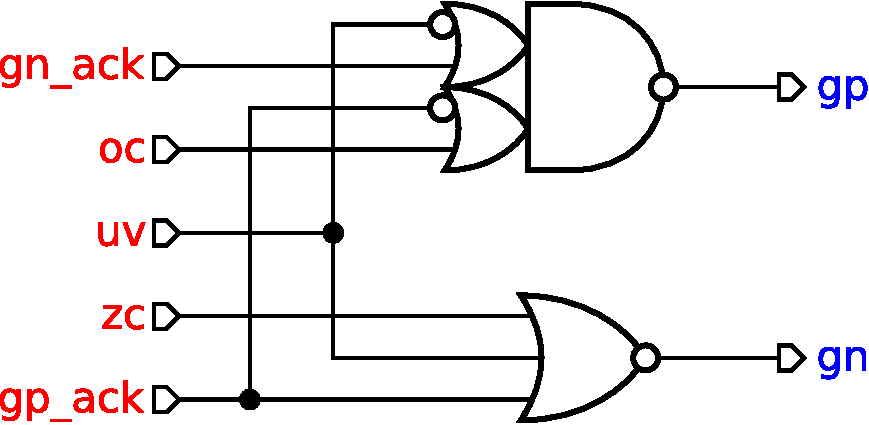
\includegraphics[scale=0.3]{Images/complex-gate-circuit-buck}
\par\end{centering}

\protect\caption{\label{fig:complex-gate-circuit}Complex gate implementation.}
\end{figure}

Complex-gate synthesis does not use a gate library and yields Boolean functions of arbitrary complexity.
These functions are often too large to be implemented by a single gate available in the gate library.
Unfortunately, breaking up a complex-gate into smaller ones, when performed na\"{\i}vely, generally yields
an incorrect circuit -- this happens due to the delays associated with the outputs of the newly introduced gates and can lead to glitches or deadlocks.

In fact, logic decomposition in the context of speed-independent circuits is a very difficult problem,
that cannot always be solved. \noun{Petrify} and \noun{MPSat} backend tools do a good job in many situations,
but occasionally they fail to converge to a solution and a manual intervention by the designer is required.

Another type of synthesis is \emph{Technology mapping}. This performs \emph{Logic decomposition} and uses a gate library to map the logic only onto gates available in the library.

\begin{figure}[h]
\begin{centering}
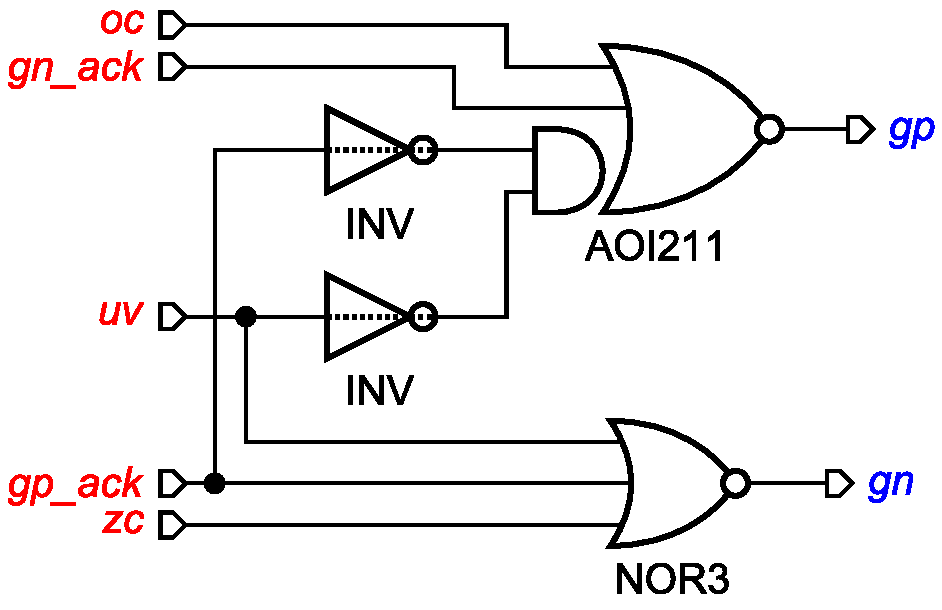
\includegraphics[scale=0.3]{Images/circuit-buck-mapped-pfy-wc.pdf}
\par\end{centering}

\protect\caption{\label{fig:tech-mapped-circuit}Technology mapped implementation.}
\end{figure}

Figure~\ref{fig:tech-mapped-circuit} is the technology mapped implementation.
The gate labels correspond to the gate names in the library.
The two inverters are shown with a dotted line through.
This is because they have the \emph{Zero delay} property expressing the assumption that their output wire delays are negligible.
This is usually unproblematic as long as such input inverters are placed close to the main gate;
this can be enforced during the place-and-route stage.

Within \noun{Workcraft} we can further decompose the implementation of $gp$ into two-input gates,
as shown in Figure~\ref{fig:circuit-buck-deco2}. This is achieved by restricting the synthesis
back end (in this case \noun{Mpsat}) to use the gates with at most two inputs.
Such 2-input decompositions may be beneficial for designs targeting low
operating voltages.

\begin{figure}[h]
\begin{centering}
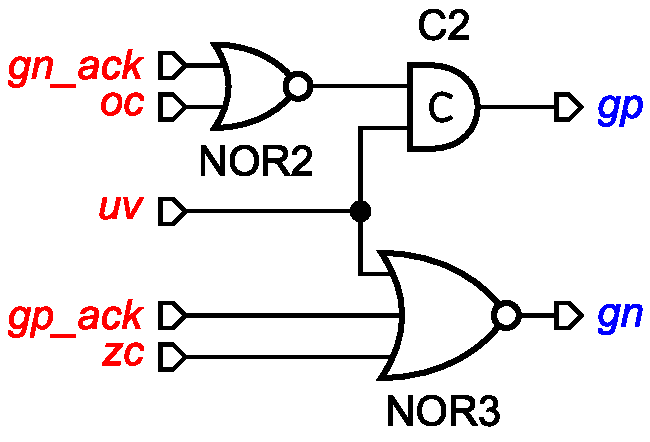
\includegraphics[scale=0.3]{Images/circuit-buck-deco2-wc}
\par\end{centering}
\protect\caption{\label{fig:circuit-buck-deco2}Technology mapping into 2-input gates/latches.}
\end{figure}

More information on the synthesis of this example can be found in the tutorials of the \noun{Workcraft} website~\cite{Workcraft_website}.

%When we have acquired a circuit design via a chosen synthesis type, it needs to be verified to
%ensure that the logic will perform as we expected before the circuit
%is fabricated. To verify this, the circuit is converted into a so-called
%circuit Petri net, using a model for each logic gate and combining
%them by means of read-arcs. By reachability analysis of this Petri
%net one can verify that the corresponding circuit is deadlock-free,
%hazard-free and conforms to the specification~\cite{2008_poliakov_async}.

%\vspace{-2mm}

\section{Related work\label{sec:related-work}}

There are several existing methodologies which are similar to the
one being proposed in this paper, and there are a common set of features between these which can be compared.
In some cases, these cannot be used for asynchronous designs, but some of their other key features can still be compared.
Table~\ref{tab:related_work} contains a comparison of these features.

We have found these related works limited in certain aspects, and we discuss this below.

\begin{table*}[t]
\caption{A comparison of features of related works and the proposed method \label{tab:related_work}}
  \centering
  \begin{tabular}[htb]{| m{2.6cm} | m{2.0cm} | m{1.3cm} | m{1.75cm} | m{1.5cm} | m{1.5cm} | m{1.7cm} | m{1.9cm} |}
  \hline
  Title             & \,Asynchronous support & \,Tool support  & \,Composition & \,Gate-level & \,Event-level & \,Protocol-level  & \,Design focus \\ \hline \hline
  Concepts            & Yes                               & Yes                  & Yes               & Yes                       & Yes                         & Yes                              & Little digital \\ \hline
  Balsa             & Yes                               & Yes                  & No                & Yes                       & No                          & Yes                              & Big digital \\ \hline
  Biscotti            & Yes                               & Yes                  & No                & Yes                       & No                          & No                               & Big digital \\ \hline
  Lava              & No                               & Yes                  & No                & Yes                       & No                          & Yes                              & Big digital \\ \hline
  C$\lambda$ash     & No                               & Yes                  & No                & Yes                       & No                          & Yes                              & Big digital \\ \hline
  Snippets          & No                                & No                   & Yes               & No                        & No                          & No                               & Little digital \\ \hline
  DI algebra        & Yes                               & No                   & Yes               & No                        & Yes                         & No                               & Little digital \\ \hline
  Structural design & No                                & Yes                  & No                & No                        & No                          & No                               & Modular \\ \hline
  \end{tabular}
  \vspace{-3mm}
\end{table*}

A common approach of designing asynchronous circuits,
\textbf{Balsa}~\cite{edwards2002balsa}, uses an RTL language to specify
operations for asynchronous circuits for both big-digital, data featuring
multiple bits, and little-digital, control systems. A Balsa specification is
initially converted into a format describing a network of handshake components,
which can be used for simulation and circuit diagrams. This can then be used in
synthesis, by mapping handshake components on to library
components~\cite{van1993handshake}. RTL languages
are used for synchronous design, and thus designers can adapt to Balsa
more easily, however specifying a control system can lead to a complicated
program which can be difficult to
comprehend, in comparison to the STGs produced in the proposed approach,
in which signal interactions can be visualised.

\textbf{Biscotti}~\cite{5232351} is an approach which uses a C-style language,
which can be easy to adapt to as designers are likely to have programming
experience. It features
\emph{forever} blocks, in which code runs sequentially, but all these
blocks run concurrently to each other. This design method starts by
specifying a circuit which is then
\emph{compiled} into a Petri-net for verification with existing tools
including \noun{Workcraft} and if successful, synthesis, similar to our
approach with conversion of concepts to allow
use with multiple existing tools based on STGs. Biscotti is aimed at
designing data-driven asynchronous systems however, and as with Balsa,
specifying an asynchronous control system is
difficult, especially as the number of signals involved increases.

\cite{bjesse1998lava} introduces \textbf{Lava}, a Haskell tool. This features its own design flow, using predefined functions for structures like logic gates, allowing users to define
functions using these structures. A collection of these functions can be used to design a circuit and be verified within Lava, however for steps such as simulation and synthesis, Lava
generates VHDL code to be used by other software. This has similar ideals to concepts, allowing users to define functions from predefined structures, which can be reused. However,
Lava is more focussed on designing synchronous circuits for data operations featuring wires with multiple bit widths, rather than asynchronous control systems. Concepts are also
focussed on more than just logic gates, and allows definitions both as standard and user-defined at multiple levels; signal-, gate-, protocol- and scenario-level.

\textbf{C$\lambda$ash}, introduced in~\cite{baaij2009clambdaash},  is also a Haskell
based tool, similar to Lava, focussed on synchronous data circuits.  It has some
cross-over features with Lava, such as built-in verification, and the ability for
users to define functions.
% Note: not sure what you mean: Clash doesn't synthesise asynchronous circuits!
% C$\lambda$ash, however, uses existing Haskell
% constructs to directly synthesize as asynchronous operations.
C$\lambda$ash also features built in synthesis and simulation, avoiding the need to export VHDL, however this feature remains. This allows a simpler way of
specifying synchronous circuits, which may be more natural for designers,
however Haskell as a language features huge differences to programming languages
like \noun{C}. The idea of a natural description is shared with Concepts,
but as with Lava, the main focus is on logic gates, and other high level descriptions, where as Concepts allow multiple levels, from low to high, when specifying.

\textbf{Snippets}~\cite{raey}, similar to concepts, are smaller
state graph models which are used to compose full state graphs of
larger systems. Snippets describe the operation of a part of a system
in terms of input and output alphabets, and in which ways these snippets
can fail. When composed with other snippets it can produce a working
system state graph model. With our design methodology however we want
to go deeper and decompose a component into concepts responsible for
capturing signal behaviours for system features, such as handshakes,
mutual exclusion, synchronisation, etc.

\textbf{DI algebra}~\cite{josephs1993overview} is a method of describing
systems as algebraic equations. Each equation represents an operation
of the specification, similar to scenarios, and composing these can
be simplified for the most compact version of the equation. These
can then be composed to find an equation for the whole specification
and again simplified for the most compact version. Our method is similar
to DI algebra, however concepts are described textually, which is
different to DI algebra and as such, simplification does not occur
at concept level, but during the composition and combination steps,
and the most compact form of the model is automatically produced.
To the best of our knowledge there are no tools or methodologies supporting
compositional design of asynchronous circuits using DI algebra and
it is therefore not interoperable with the rest of our design flow,
and this also makes it unsuitable for use in an industrial setting.

\textbf{Structural design} features re-usability of modular components~\cite{modular-circuit-design}.
Here, a component design can be used multiple times across full device
designs in conjunction with several other circuit modules. These modules
can be changed in some way without affecting how they are used in
the full device designs. The ideas of this method are similar to that
of the design methodology we are proposing to reduce design time.
However, this method is at a much higher level, using fully designed
and tested components where as we propose to allow re-usability when
modelling at circuit level, using composed concepts.

Concepts have many advantageous features, such as reuse, natural description, multiple level description and composition, and more.
Several of these approaches feature similar ideas which make them beneficial in certain ways,
but we believe fall down where the inclusion of one or more of these features could make an approach better. With concepts,
we have attempted to address these issues and make concepts not only a powerful tool to specify asynchronous circuits, but a method with as much ease-of-use as possible, particularly targeting the little-digital design domain.
Concepts are also supported by industrial-strength open-source software
toolsuite \noun{Workcraft}.

%\textbf{Resynthesis}~\cite{Resynth2} is a process of decomposing
%a full model and recomposing it of selective components to produce
%a smaller model. This can be used to reduce the number of signals
%to connect two separate models for example. This process is regularly
%used for optimisation of Balsa control circuits~\cite{plana2005attacking},
%however in Balsa the set of predefined components is fixed, so a designer
%cannot easily introduce new scenarios. Resynthesis also requires full
%models which can be decomposed. This requirement may be problematic
%for the proposed methodology as we take a ground-up approach to composition,
%starting with primitive concepts which composed into scenarios, which
%are subsequently combined into a complete model. Resynthesis can still
%be used at a later stage of the design process, once the complete
%model of a system~(or a subsystem) has been obtained using the proposed
%methodology.

\section{Conclusions and future work\label{sec:conclusions}}

In this work we show that it is possible to design asynchronous control
circuits at the interface between analogue and digital worlds by
splitting their specification into operational modes, scenarios, and
describing signal interactions and requirements of each scenario using
high-level asynchronous concepts. These can then be translated into STGs
that represent these operational modes, which can be used with existing
verification and synthesis tools. STGs can be further combined to
produce a complete model for the system specification.

Using concepts, a user can reduce the time of designing an asynchronous
control circuit from the ground up, as well as allow reuse of components
either as part of a scenario or entire scenarios to reduce the design-time
of future projects. Composition of concepts and scenarios can help
reduce errors and save time in comparison to performing these manually.
This method can help to make asynchronous circuits more appealing
to industrial designers.

Currently, this method works with Signal Transition Graphs, however
it can be applied to other modelling disciplines, such as Finite State
Machines~(FSM).

\emph{Process mining} can also be used for various purposes in conjunction
with designing asynchronous circuits. For example, process mining can discover a
behavioural model when none exists, and can be used to check that an existing
specification is realistic, or find less complex models. All of this can be
performed automatically, by tools such as \noun{PGminer}~\cite{mokhov2016mining}, given
an event log with observations of a real analogue or digital system, and aid a
designer in reducing design time and errors. We aim to include process mining
in the design flow for the proposed approach.

% We aim to test concepts using examples from several different areas where
% asynchronous circuits are beneficial.
% These will be of various sizes, featuring differing numbers of signals, in an attempt to find problematic areas of the concepts design methodology.
% We can then use this information to imporove concepts.

As the Internet-of-Things becomes ubiquitous, asynchronous circuits
will be key in designing energy-efficient and reliable IoT nodes,
particularly at the interfaces between analogue and digital domains,
such as power management units. We believe that high-level asynchronous
concepts could be instrumental in the design of these systems.

%CPOG and Parameterised Graph models are also integrated into
%\noun{Workcraft}~\cite{Workcraft_website} as part of the \noun{Scenco} toolsuite~\cite{2015_workcraft_scenco}~\cite{Scenco_paper},
%allowing circuits to be described by algebraic equations in text
%form. \noun{Scenco} provides support for describing concept models
%to produce scenarios and then compose scenarios to produce full system
%implementations.

%In certain cases, an implementation may need to be changed based on
%design parameters to produce the best result, and these may change
%during run-time or after the fabrication stage. CPOGs support parameter
%and run-time reconfigurability~\cite{microadapt}, hence if
%design parameters change, the design does not need to be recomposed
%from another list of concepts, thus saving time. For this reason,
%CPOGs could work very well with this design approach.


%
%In certain cases, an implementation may need to be changed based on
%design parameters to produce the best result, and these may change
%during run-time or after the fabrication stage. CPOGs support parameter
%and run-time reconfigurability~\cite{microadapt}, hence if
%design parameters change, the design does not need to be recomposed
%from another list of concepts, thus saving time. For this reason,
%CPOGs could work very well with this design approach.

%STGs and CPOGs both have their benefits when working with asynchronous
%systems, and it will be useful to compare these two methods, to see
%if either is better when designing a system from concepts, or see
%if there are certain specifications where one modelling method is
%better than the other. It may be necessary to have a form of interaction between CPOGs and STGs in order to provide a more streamlined method of designing asynchronous circuits
%using concepts, and this is something we aim to explore.

%\vspace{-2mm}

%
%In addition to FSMs and STGs, we also plan to extend this design method
%to support Conditional Partial Order Graphs~(CPOGs)~\cite{CPOG1}
%and Parameterised Graphs~\cite{mokhov2014algebra} for modelling
%asynchronous circuits. These models are also integrated into \noun{Workcraft}
%as part of the \noun{Scenco} toolsuite\noun{~\cite{2015_workcraft_scenco},
%}allowing circuits to be described by algebraic equations in text
%form. \noun{Scenco} provides support for describing concept models
%to produce scenarios and then compose scenarios to produce full system
%implementations.
%
%CPOGs can also be used for process mining, using tools such as \noun{PGminer}~\cite{mokhov_2016_mining, pgminer}.
%Process mining can be used for various purposes in conjunction with designing asynchronous circuits. For example, process mining can find a behavioural model if non exists, and can be
%used to check that an existing specification is realistic, or find less complex model. All of this can be performed automatically, and aid a designer in reducing design time and errors.
%

%\vspace{-3mm}

\section*{Acknowledgements}

%\vspace{-2.5mm}

The authors would like to thank the reviewers for their constructive
comments. This research is supported by EPSRC research grant `A4A:
Asynchronous design for Analogue electronics' (EP/L025507/1) and
the Royal Society research grant `Computation Alive: Design of a
Processor with Survival Instincts'.

%\vspace{-2.5mm}

\bibliographystyle{unsrt}
\bibliography{publications}

\end{document}
